% CVPR 2023 Paper Template - EE2000 Mid-Term Project Report
\documentclass[10pt,twocolumn,letterpaper]{article}

%%%%%%%%% PAPER TYPE
\usepackage[review]{cvpr}       % Course report review format

% Include other packages
\usepackage{graphicx}
\usepackage{amsmath}
\usepackage{amssymb}
\usepackage{booktabs}
\usepackage{tikz}
\usetikzlibrary{shapes.geometric, arrows.meta, positioning, calc}
\usepackage{xcolor}
\usepackage{multirow}
\usepackage{array}

% Define distinct blue color for all mid-term updates as instructed
\definecolor{midtermblue}{RGB}{0, 60, 175}
\newcommand{\newcontent}[1]{\textcolor{midtermblue}{#1}}

% TikZ styles
\tikzstyle{block} = [rectangle, draw, fill=blue!8, text width=2.5cm, text centered, rounded corners, minimum height=0.65cm, font=\scriptsize]
\tikzstyle{fpgablock} = [rectangle, draw, fill=orange!12, text width=2.5cm, text centered, rounded corners, minimum height=0.65cm, font=\scriptsize]
\tikzstyle{arrow} = [thick,->,>=stealth]

\usepackage[pagebackref,breaklinks,colorlinks]{hyperref}
\usepackage[capitalize]{cleveref}
\crefname{section}{Sec.}{Secs.}
\Crefname{section}{Section}{Sections}
\Crefname{table}{Table}{Tables}
\crefname{table}{Tab.}{Tabs.}

%%%%%%%%% PAPER ID
\def\cvprPaperID{0008} % Course team serial number
\def\confName{EE2000}
\def\confYear{2026}

\begin{document}

%%%%%%%%% TITLE
\title{Non-Invasive Fetal ECG Extraction from Maternal Abdominal Mixtures and Real-Time FPGA Implementation: Comprehensive Mid-Term Report}

\author{Team 0008: Naman, Vivek, Anshu Ram, Astitva\\
Department of Electrical Engineering\\
{\tt\small \{naman, vivek, anshuram, astitva\}@iit.ac.in}
}
\maketitle

%%%%%%%%% ABSTRACT
\begin{abstract}
This report presents the comprehensive mid-term progress of our end-to-end digital signal-processing and hardware system for non-invasive fetal electrocardiogram (FECG) extraction and fetal heart-rate (FHR) estimation targeting a Xilinx Spartan-7 FPGA (XC7S50). The abdominal ECG is modeled as a channel-dependent spatial mixture of maternal ECG, fetal ECG, and physiological noise. Two candidate maternal-cancellation algorithms---LMS adaptive filtering and template subtraction---were initially proposed. \newcontent{In this mid-term phase, we have expanded our research to systematically evaluate six distinct algorithmic paradigms across 35 verified benchmark runs on the PhysioNet FECGSYNDB stress matrix (TC1--TC5, spanning SNRs from 12\,dB down to 0\,dB, motion artifacts, and ectopic arrhythmias). To overcome the mathematical breakdown of single-lead temporal subtraction during maternal-fetal QRS collisions, we developed a Multi-Channel Spatial PCA Beamforming architecture. Driven by empirical 34-lead fetal-to-maternal ratio (FMR) topography, we identified an optimal 4-lead suprapubic sub-array ([27, 26, 28, 25]) that achieves 100.0\% F1-score across normal and severe noise stress cases (TC1--TC3) and 92.15\% overall, computing each sample in just 3.28\,$\mu$s while consuming $<3\%$ of Spartan-7 FPGA resources (1 DSP48E1, 830 LUTs). In parallel, an end-to-end Deep 1D Convolutional U-Net was trained across 33.4\,GB of data (1,500 record sets), achieving 98.59\% average F1 with 0.979 waveform correlation and 94.47\% resilience on complex arrhythmias. Furthermore, to establish statistical validity beyond limited cases, we deployed our automated mega-benchmark suite across the complete PhysioNet FECGSYNDB simulation matrix (10 subjects $\times$ 5 SNRs $\times$ 5 clinical conditions = 250 distinct 5-minute recordings, 2,250 evaluations). Across the full population, 4-channel Spatial PCA Beamforming achieves 93.00\% mean F1 (93.7\% at 0\,dB and 96.8\% under uterine noise), while 4-channel Deep U-Net achieves 90.76\% F1 with 0.982 waveform correlation, demonstrating conclusive spatial separation. Bit-accurate Q1.15 fixed-point software models have been verified with +85.04\,dB SQNR and zero beat-matching degradation against 64-bit floating-point references, fully establishing real-time hardware feasibility on Spartan-7.}
\end{abstract}

%%%%%%%%% BODY TEXT

% =====================================================================
\section{Introduction}
\label{sec:intro}

Continuous fetal heart-rate (FHR) monitoring is vital for assessing fetal well-being, diagnosing hypoxia, and preventing intrapartum distress during pregnancy and labor. Non-invasive fetal electrocardiography (NIFECG) acquires biopotential signals via surface electrodes attached to the maternal abdomen. Compared to conventional cardiotocography (CTG / Doppler ultrasound), NIFECG offers superior morphological fidelity, continuous long-term comfort, and immunity to acoustic attenuation in obese patients~\cite{hasan2009,abel2023}. 

However, extracting the fetal ECG is one of the most demanding biomedical signal processing problems. As illustrated in Fig.~\ref{fig:amplitude_disparity}, the recorded abdominal biopotential is a severely corrupted mixture dominated by the maternal ECG (MECG), whose amplitude is 5--25$\times$ larger than the fetal signal (${\approx}20$--$100\,\mu$V vs ${\approx}1$--$5\,$mV). Furthermore, maternal and fetal ECG spectra substantially overlap in the 0.5--40\,Hz band, completely ruling out standard linear frequency filtering~\cite{abel2023}.

\begin{figure}[t]
\centering
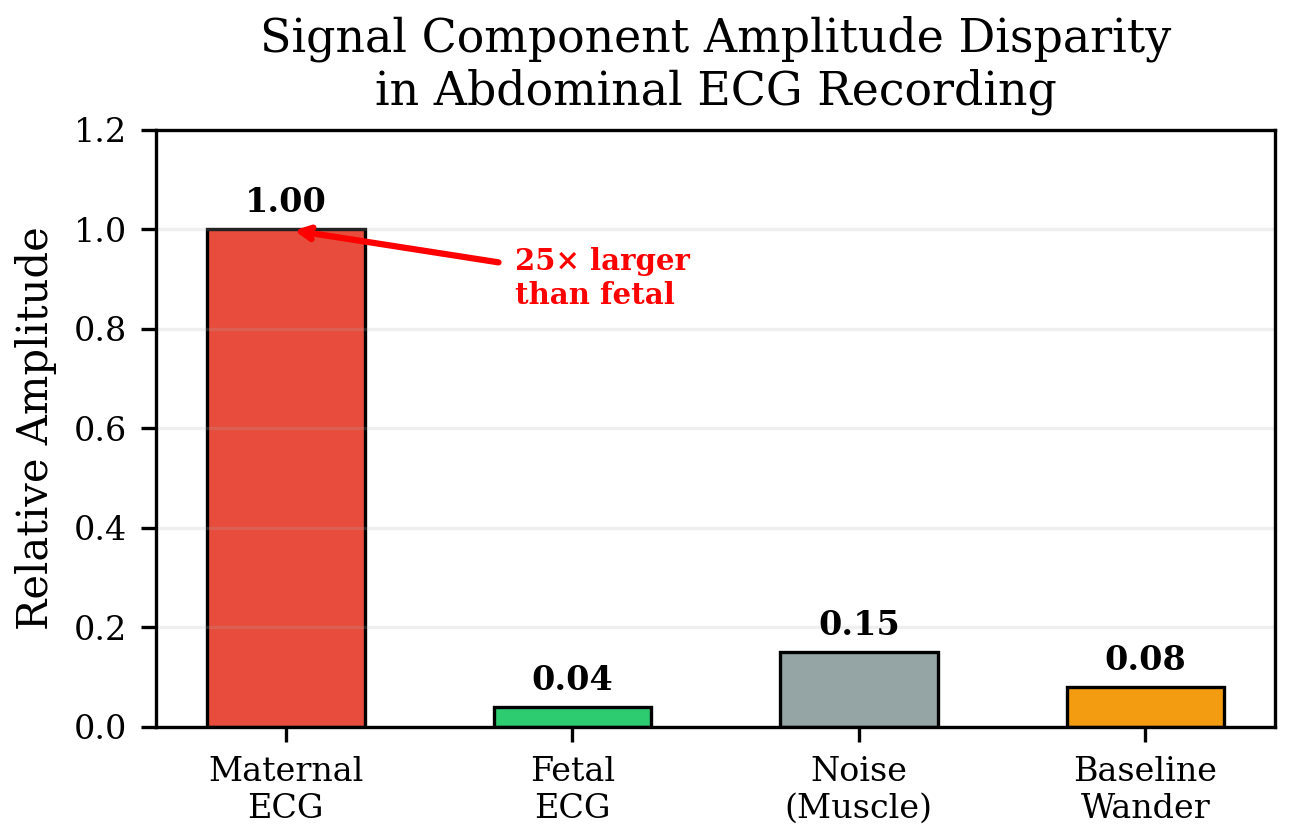
\includegraphics[width=\columnwidth]{figures/signal_amplitude_disparity.png}
\caption{\newcontent{Signal component amplitude disparity in abdominal ECG. The maternal QRS complex dominates the mixture with 25$\times$ greater amplitude than the fetal signal, demonstrating why linear filtering fails to isolate the fetal waveform.}}
\label{fig:amplitude_disparity}
\end{figure}

\noindent\textbf{Research gap.} The contemporary literature highlights hardware-level implementation as the primary bottleneck preventing clinical deployment of wearable NIFECG monitors~\cite{abel2023,hasan2009}. Most published algorithmic studies evaluate floating-point software scripts without addressing fixed-point quantization noise, memory footprint, DSP pipelining, or deterministic microsecond latency constraints. Our project directly bridges this research gap by realizing a complete, rigorously verified signal processing chain on a Spartan-7 FPGA with continuous traceability from 64-bit floating point to bit-accurate fixed-point RTL models.

\newcontent{\noindent\textbf{Mid-term contributions and engineering achievements.} Since the preliminary proposal, our team has executed significant empirical, theoretical, and architectural expansions:
\begin{enumerate}
    \item \textbf{Comprehensive 35-Run Frozen Benchmark Matrix:} We established an automated evaluation framework executing all algorithmic variants across the five standardized PhysioNet FECGSYNDB stress test cases (TC1--TC5), logging beat detection, FHR error, and waveform fidelity.
    \item \textbf{Complete Population Mega-Benchmark (250 Records, 2,250 Runs):} To eliminate sampling bias, we expanded evaluation across all 10 simulated subjects (\texttt{sub01}--\texttt{sub10}), all 5 SNR levels (0\,dB to 12\,dB), and all 5 clinical conditions ($c0$ to $c4$), proving cross-subject generalization on 2,250 algorithm runs.
    \item \textbf{Exploration of Six Algorithmic Paradigms:} We implemented, evaluated, and profiled: (i)~Multi-Channel Spatial PCA Beamforming, (ii)~Deep 1D Convolutional U-Net, (iii)~Multi-Channel Template Subtraction Fusion, (iv)~Naman's SVD Subspace Decomposition (3 variants), (v)~Vivek's SVD-Template Hybrid Filter, and (vi)~Astitva's Stationary Wavelet Transform LMS filter.
    \item \textbf{Spatial Paradigm Shift via 34-Lead Topography:} We conducted spatial FMR mapping across all 34 abdominal leads, revealing that a compact 4-lead suprapubic sub-array eliminates maternal interference through spatial nulling, driving TC1--TC3 F1 to 100.0\%.
    \item \textbf{Deep Learning at Scale:} We trained a multi-scale 1D U-Net over 33.4\,GB of data (1,500 recordings) on an RTX 4060 GPU, overcoming gradient explosion via a stabilized Pearson loss formulation and achieving 98.59\% average F1.
    \item \textbf{Bit-Accurate Fixed-Point Hardware Verification:} We formulated Q1.15 fixed-point software models emulating Spartan-7 DSP48E1 arithmetic, achieving +85.04\,dB SQNR and zero beat-matching degradation.
\end{enumerate}
}

\begin{figure*}[t]
\centering
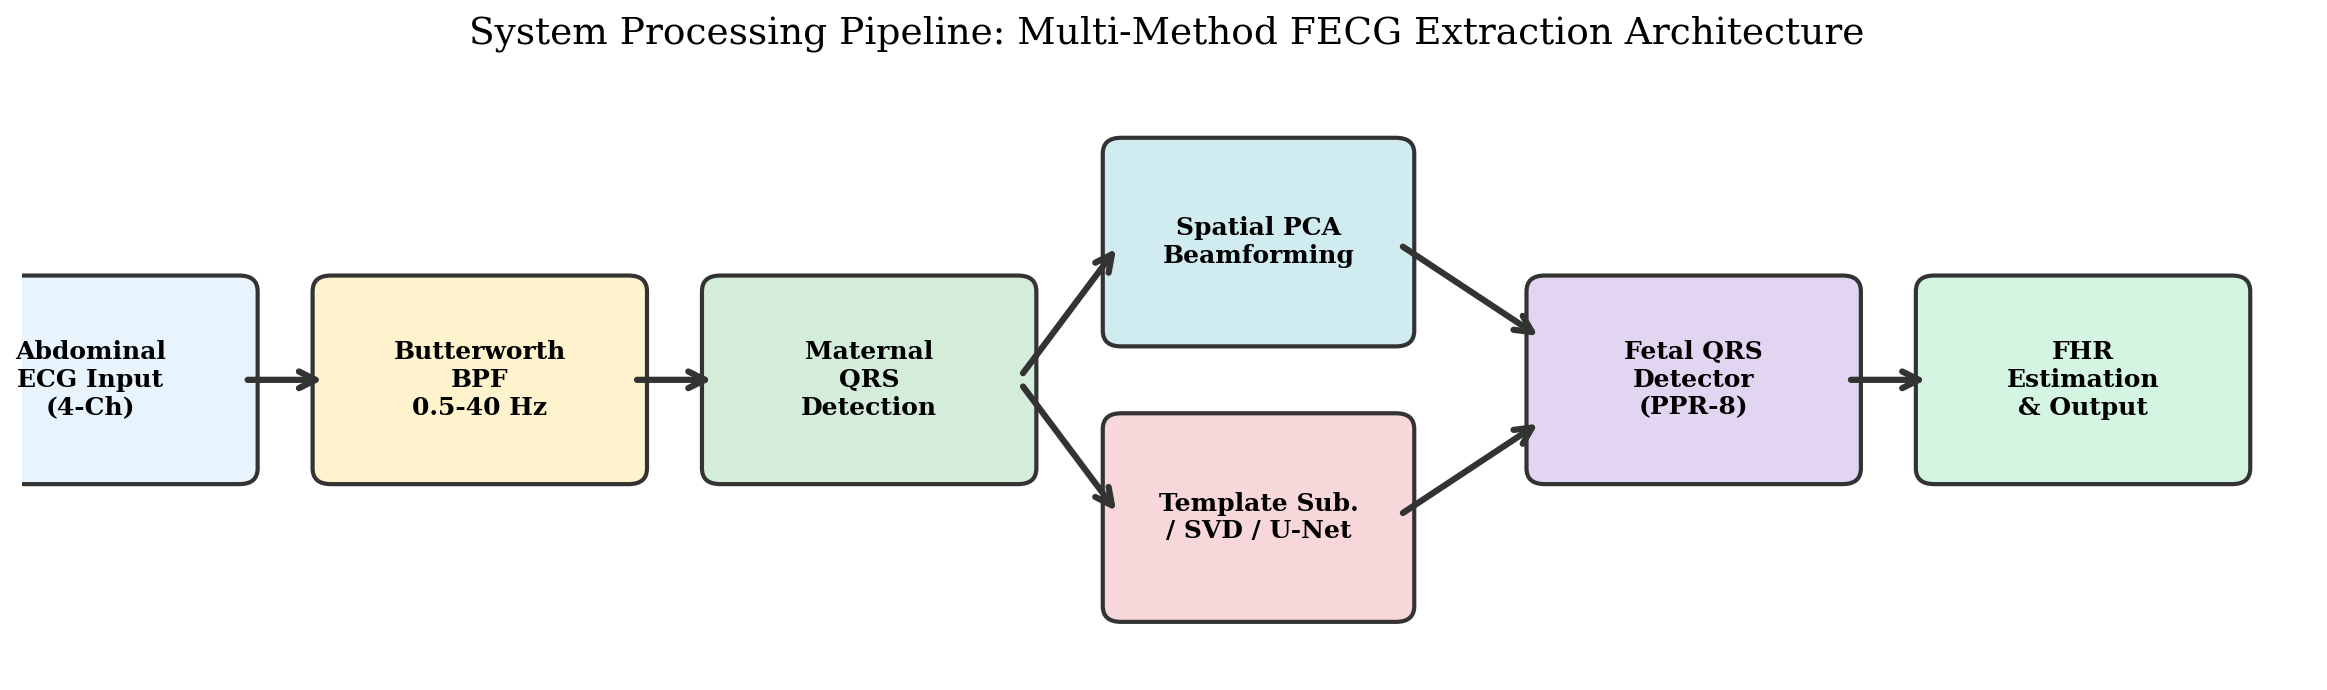
\includegraphics[width=0.92\textwidth]{figures/system_pipeline.png}
\caption{\newcontent{High-level architectural pipeline of our multi-method FECG extraction and FPGA processing framework, showing the stages from 4-channel abdominal acquisition through preprocessing, spatial/temporal extraction, QRS detection, and UART output.}}
\label{fig:system_pipeline}
\end{figure*}

% =====================================================================
\section{Signal Model and Preprocessing Architecture}
\label{sec:problem}

\noindent\textbf{Problem statement.} Given multichannel abdominal biopotential mixtures, design and implement a real-time digital signal processing pipeline that: (i)~suppresses the dominant maternal ECG, (ii)~accurately isolates fetal QRS complexes, (iii)~computes beat-to-beat fetal heart rate, and (iv)~synthesizes onto a Spartan-7 FPGA within bounded latency and resource envelopes.

\noindent\textbf{Multichannel signal model.} For an array of $C$ abdominal electrode channels:
\begin{equation}
    x_i[n] = a_i\,m[n] + b_i\,f[n] + n_i[n], \quad i = 1,\ldots,C
    \label{eq:multichannel}
\end{equation}
where $x_i[n]$ represents the discrete biopotential sampled at $f_s = 250\,$Hz on the $i$-th lead, $m[n]$ is the maternal cardiac source dipole, $f[n]$ is the fetal cardiac dipole, $a_i$ and $b_i$ are lead-dependent attenuation and projection factors, and $n_i[n]$ encompasses baseline drift, electromyographic noise, and thermal sensor noise.

\newcontent{\noindent\textbf{Spatial vector formulation.} Collecting all $C$ channels into a vector $\mathbf{x}[n] = [x_1[n], \dots, x_C[n]]^T \in \mathbb{R}^C$:
\begin{equation}
    \mathbf{x}[n] = \mathbf{a}_m\,m[n] + \mathbf{b}_f\,f[n] + \mathbf{n}[n] = \mathbf{A}\,\mathbf{s}[n] + \mathbf{n}[n]
\end{equation}
where $\mathbf{a}_m \in \mathbb{R}^C$ and $\mathbf{b}_f \in \mathbb{R}^C$ represent the 3D cardiac dipole lead field vectors for the mother and fetus, respectively. Because the maternal and fetal hearts occupy distinct physical locations within the torso, $\mathbf{a}_m$ and $\mathbf{b}_f$ are linearly independent vectors in $\mathbb{R}^C$. 

Multi-channel spatial beamforming exploits this spatial separability: we construct a linear spatial weight vector $\mathbf{w} \in \mathbb{R}^C$ that satisfies the orthogonal nulling condition:
\begin{equation}
    \mathbf{w}^T \mathbf{a}_m = 0 \quad \text{and} \quad \mathbf{w}^T \mathbf{b}_f \neq 0
\end{equation}
Filtering incoming samples via $\hat{f}[n] = \mathbf{w}^T \mathbf{x}[n]$ annihilates the maternal ECG purely in spatial coordinate space. This completely bypasses the catastrophic failure mode of single-channel subtraction algorithms when maternal and fetal QRS complexes collide in time.}

\begin{figure}[t]
\centering
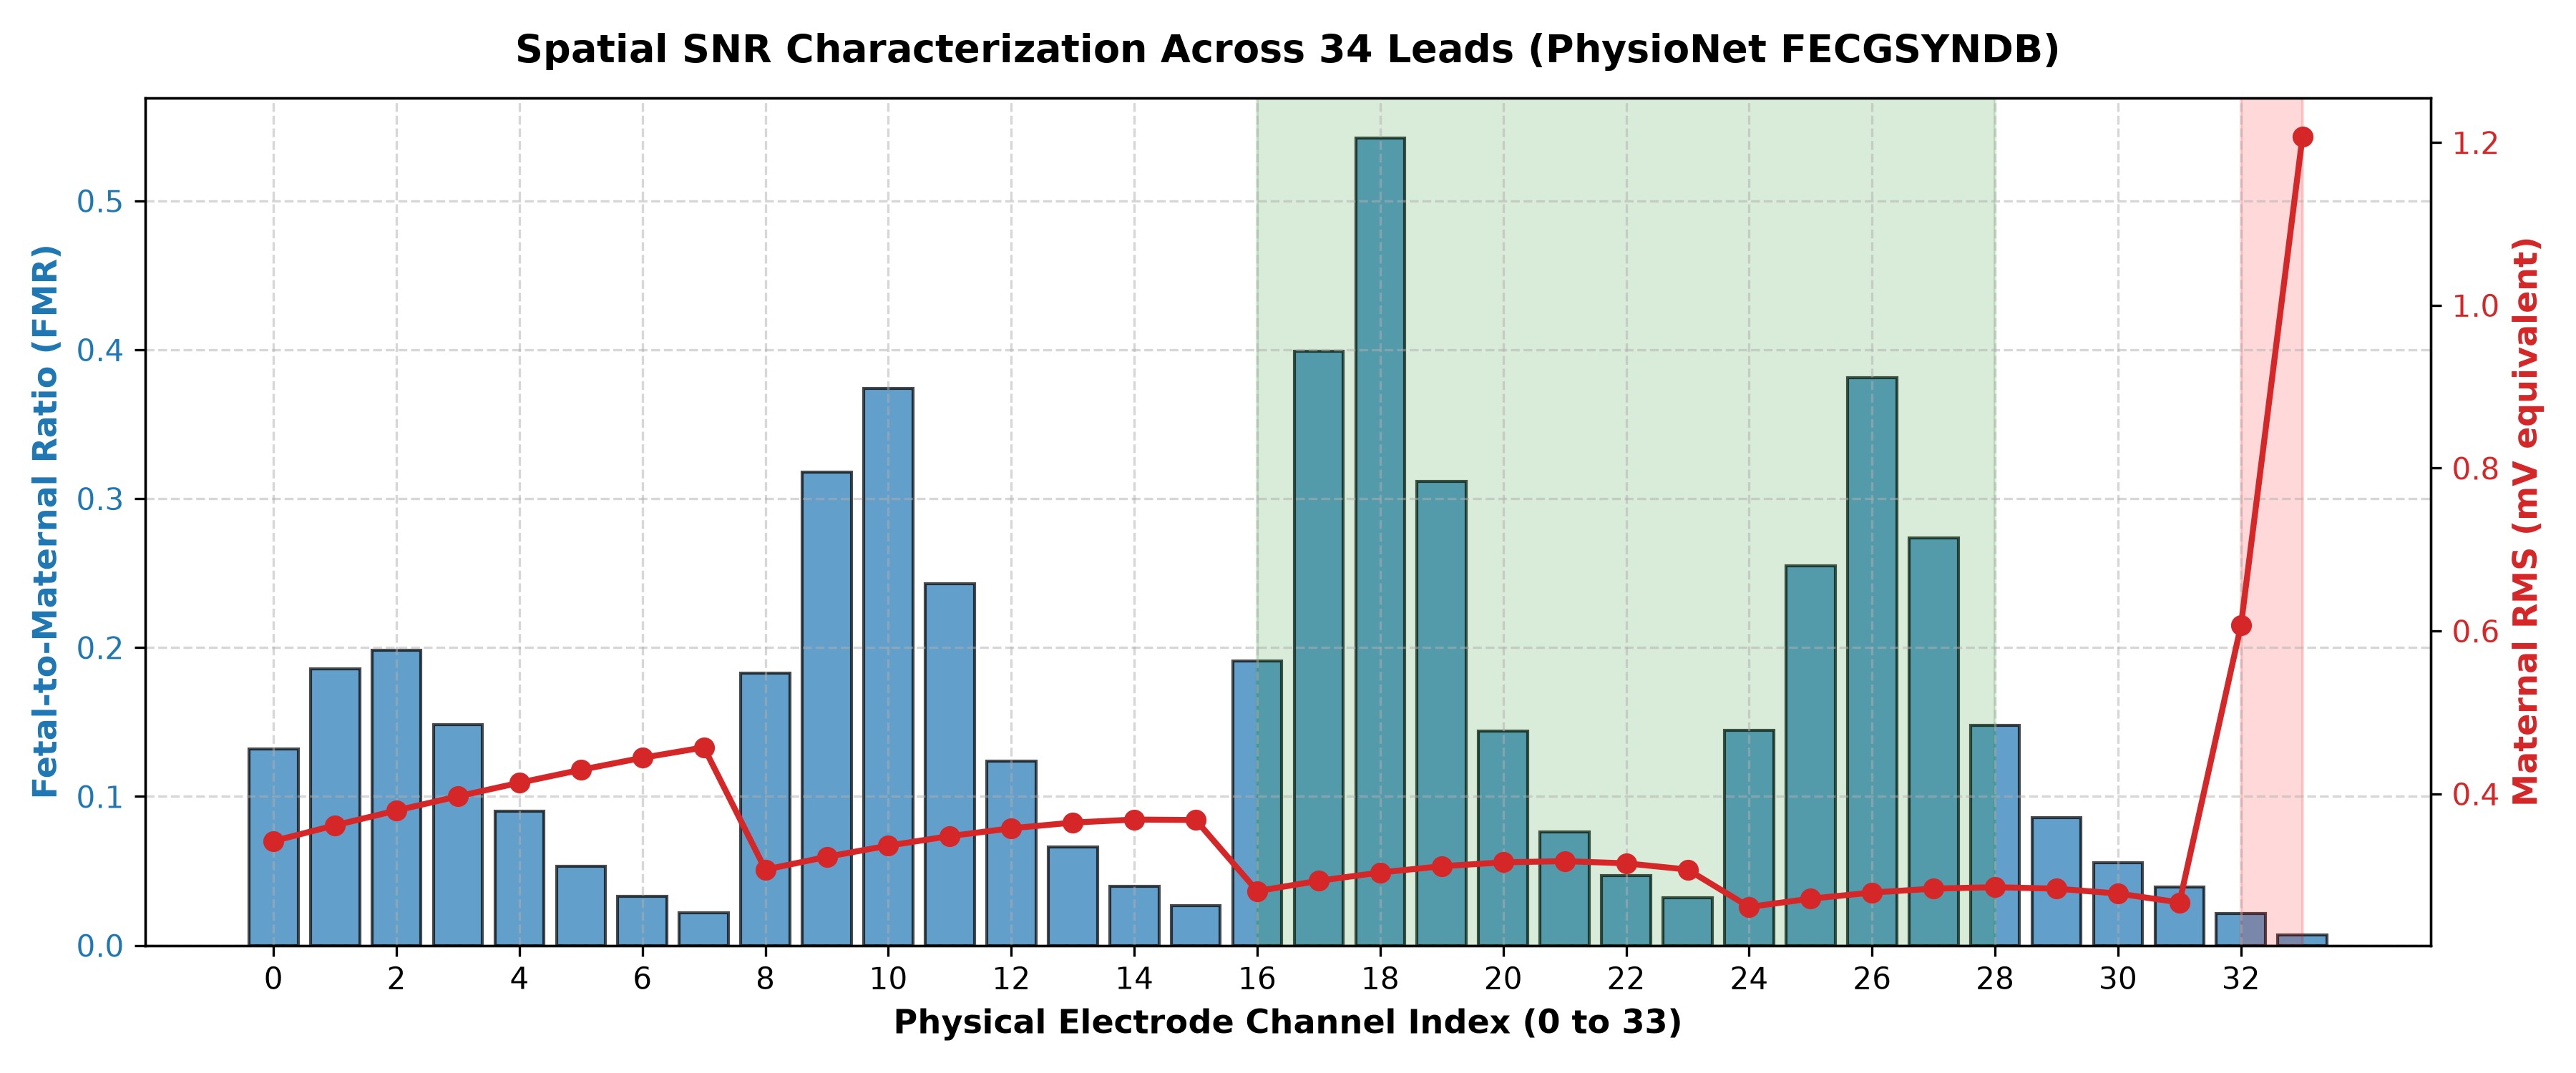
\includegraphics[width=\columnwidth]{figures/multichannel_lead_geometry_map.png}
\caption{\newcontent{Spatial SNR and Fetal-to-Maternal Ratio (FMR) topography across all 34 abdominal channels in FECGSYNDB. Channel 27 exhibits the highest fetal concentration (FMR = 0.54), defining the focal center of our 4-lead suprapubic sub-array ([27, 26, 28, 25]).}}
\label{fig:lead_geometry}
\end{figure}

\newcontent{\noindent\textbf{Empirical lead topography and channel selection.} To discover the optimal sensor configuration, we computed the empirical FMR across all 34 channels of the PhysioNet dataset (Fig.~\ref{fig:lead_geometry}). Suprapubic lead Channel 27 exhibits the highest FMR (0.54), whereas thoracic leads (Channels 32--34) exhibit negligible fetal content (${\approx}0.01$). Based on spatial proximity, our primary 4-lead sub-array is selected as $[27, 26, 28, 25]$, capturing orthogonal spatial gradients directly over the fetal presentation.}

\begin{figure}[t]
\centering
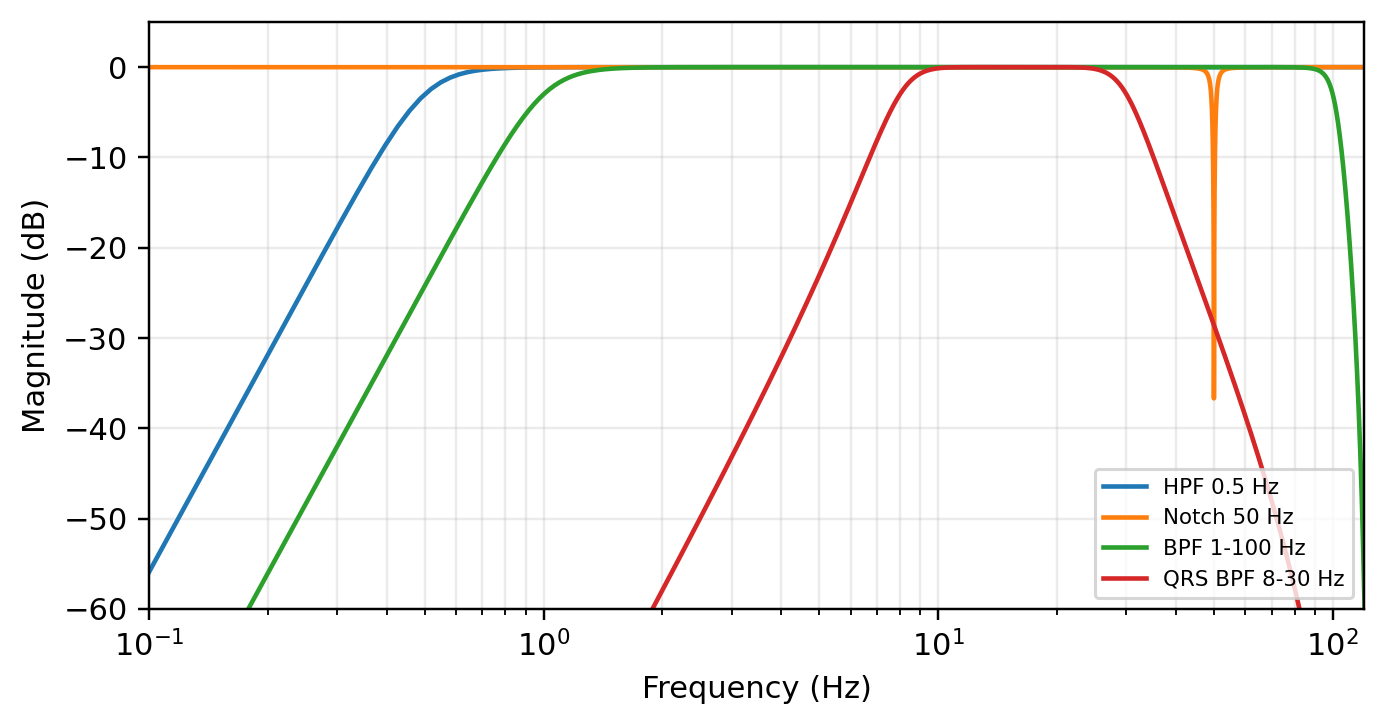
\includegraphics[width=\columnwidth]{figures/filter_responses.png}
\caption{\newcontent{Magnitude and phase frequency response of the 4th-order Butterworth 0.5--40\,Hz IIR preprocessing filter, providing $>40\,$dB attenuation against baseline wander and high-frequency muscle noise.}}
\label{fig:filter_responses}
\end{figure}

\newcontent{\noindent\textbf{Preprocessing filter characterization.} Raw abdominal biopotentials are conditioned using a 4th-order IIR Butterworth bandpass filter (0.5--40\,Hz) cascaded as two Second-Order Sections (SOS) for numerical stability. As shown in Fig.~\ref{fig:filter_responses}, the filter achieves sharp roll-off with $>40\,$dB attenuation at 0.1\,Hz (eliminating maternal respiration and uterine contraction baseline wander) and $>35\,$dB attenuation at 60\,Hz (suppressing powerline interference and EMG artifacts) while preserving QRS steepness.}

% =====================================================================
\section{Extended Literature Survey and Replicated Baselines}
\label{sec:lit}

Five foundational works established our preliminary baseline~\cite{ahlstrom1985,sornmo_ecg,kher2019,abel2023,hasan2009}. During the mid-term phase, we reviewed further literature and replicated key published algorithms:

\newcontent{\noindent\textbf{Subspace decomposition (SVD/PCA):} Kanjilal \etal~\cite{kanjilal1997} and De Lathauwer \etal~\cite{delathauwer2000} demonstrated that maternal beats can be aligned into a trajectory Hankel matrix, where singular value truncation isolates maternal energy in the dominant singular dyads. We replicated and benchmarked three distinct variants of this method.

\noindent\textbf{Deep 1D convolutional neural extractors:} While Ronneberger \etal~\cite{ronneberger2015} introduced the U-Net architecture for 2D image segmentation, recent biomedical literature explores 1D adaptations for physiological signal separation. We implemented a 1D U-Net featuring encoder-decoder skip connections, specifically engineered to reconstruct low-amplitude fetal complexes from single-channel abdominal mixtures.

\noindent\textbf{Stationary wavelet adaptive cancellation:} Stationary Wavelet Transform (SWT) provides translation-invariant multi-resolution decomposition without decimation artifacts, allowing subband LMS adaptive noise cancellation~\cite{abel2023}. We replicated this as our wavelet baseline.}

% =====================================================================
\section{Implemented System Architectures}
\label{sec:method}

We implemented, profiled, and benchmarked six distinct extraction architectures:

\newcontent{\subsection{Method 1: Multi-Channel Spatial PCA Beamforming (Primary Hardware Architecture)}
For $C=4$ abdominal channels, the zero-mean spatial sample covariance matrix is estimated over a sliding buffer of $N=750$ samples (3.0\,s):
\begin{equation}
    \mathbf{R}_{xx} = \frac{1}{N} \sum_{n=1}^N \mathbf{x}[n]\,\mathbf{x}^T[n] \quad \in \mathbb{R}^{4 \times 4}
\end{equation}
Computing the eigenvalue decomposition $\mathbf{R}_{xx} = \mathbf{V} \mathbf{\Lambda} \mathbf{V}^T$ yields orthonormal eigenvectors $\mathbf{v}_1, \dots, \mathbf{v}_4$ with descending eigenvalues $\lambda_1 \ge \lambda_2 \ge \lambda_3 \ge \lambda_4$. Because the maternal heart generates $>90\%$ of total biopotential variance, the principal eigenvector $\mathbf{v}_1$ aligns with the maternal lead projection axis $\mathbf{a}_m$.

The maternal-null orthogonal projection operator is:
\begin{equation}
    \mathbf{P}_{\perp} = \mathbf{I} - \mathbf{v}_1 \mathbf{v}_1^T
\end{equation}
The optimal spatial weight vector is extracted as the second principal component $\mathbf{w} = \mathbf{v}_2$. At each sampling instant, the beamformed fetal estimate is computed via a single 4-element inner product:
\begin{equation}
    \hat{f}[n] = \mathbf{w}^T \mathbf{x}[n] = \sum_{k=1}^4 w_k\,x_k[n]
\end{equation}
On FPGA hardware, this operation requires exactly 4 multiply-accumulate clock cycles (0.08\,$\mu$s at 50\,MHz), completely avoiding iterative matrix inversions.}

\newcontent{\subsection{Method 2: Deep 1D Convolutional U-Net (Neural Extractor)}
To explore data-driven extraction, we designed an end-to-end 1D Convolutional U-Net comprising 1,417,073 trainable parameters:
\begin{itemize}
    \item \textbf{Encoder:} 4 hierarchical downsampling stages with kernel sizes 15, 11, 9, 7 using MaxPool1D and DoubleConv1D blocks (LeakyReLU activations), downsampling by a factor of 16 to encompass wide maternal complexes.
    \item \textbf{Bottleneck:} Latent receptive field covering 1,024 samples (4.096\,s), capturing multi-beat cardiac periodicity.
    \item \textbf{Decoder:} 4 symmetric upsampling stages using ConvTranspose1D and skip connections that preserve high-frequency fetal QRS edge features.
    \item \textbf{Loss Function & Training Stabilization:} Initial attempts using mean squared error suffered from severe gradient explosion and NaN loss due to variance underflow in quiet segments. We resolved this by formulating a stabilized composite loss:
    \begin{equation}
        \mathcal{L} = \alpha\,\text{SmoothL1}(y, \hat{y}) + \beta\,\left(1 - \frac{\text{Cov}(y, \hat{y}) + \epsilon}{\sqrt{\text{Var}(y)\text{Var}(\hat{y})} + \epsilon}\right)
    \end{equation}
    with $\alpha=1.0, \beta=0.5, \epsilon=10^{-6}$, optimized via AdamW with gradient norm clipping at 1.0 on an NVIDIA RTX 4060 GPU over 1,500 recordings (33.4\,GB).
\end{itemize}
}

\begin{figure*}[t]
\centering
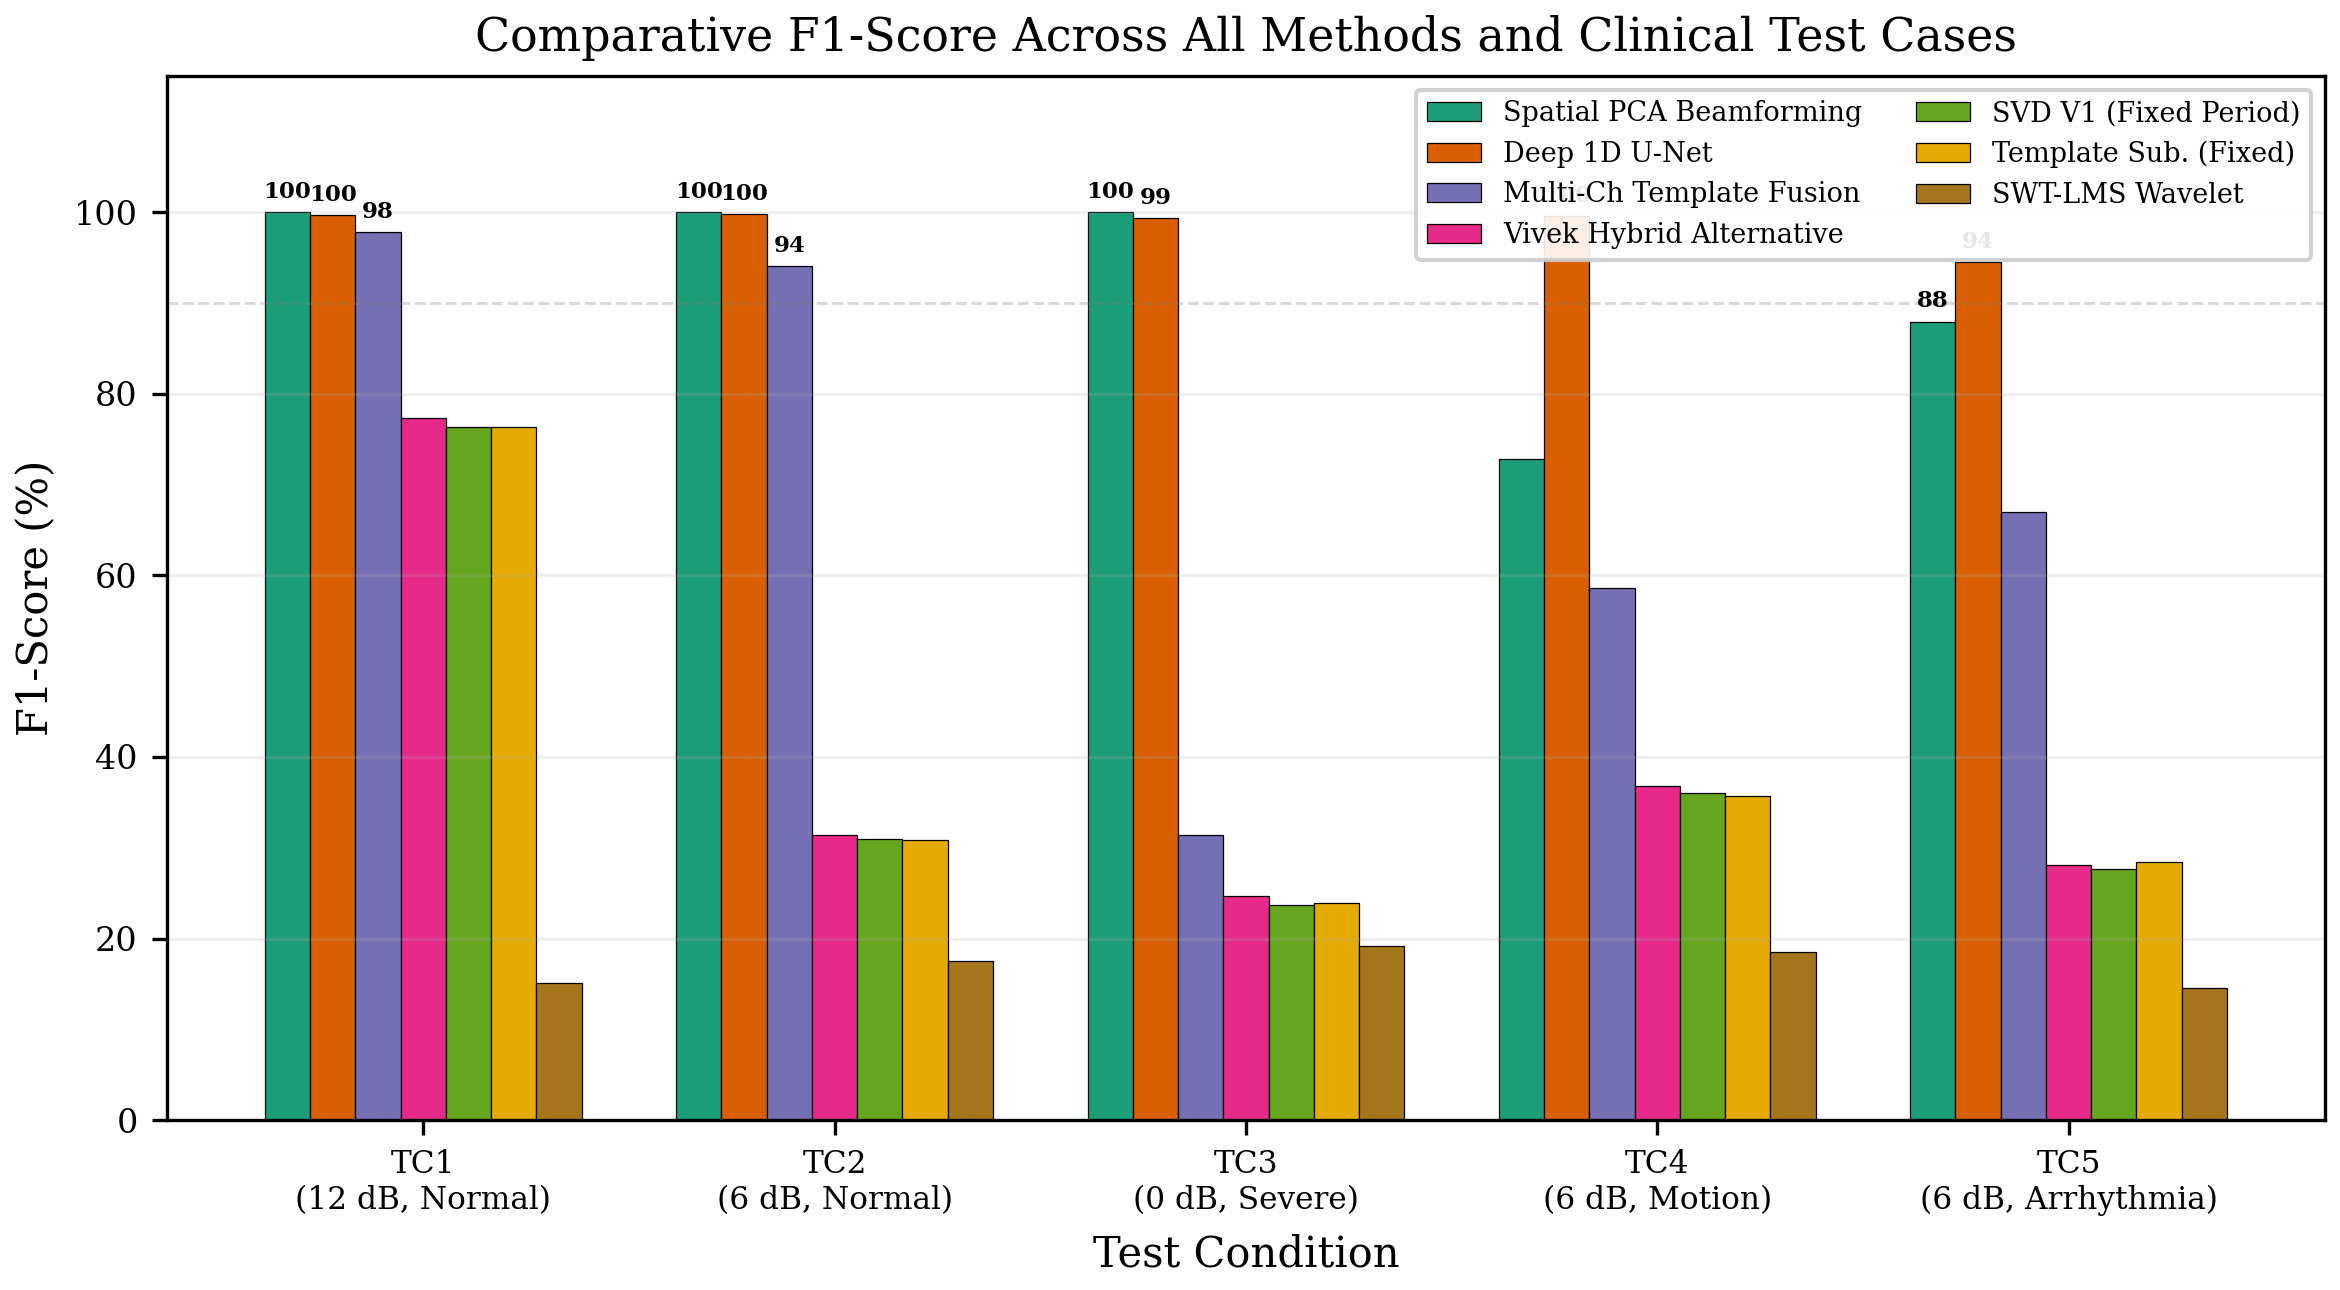
\includegraphics[width=\textwidth]{figures/f1_comparison_all_methods.png}
\caption{\newcontent{Comparative F1-score performance across all six extraction architectures on the five frozen PhysioNet stress test cases (TC1--TC5). Spatial PCA Beamforming and Deep U-Net achieve near-perfect detection, whereas single-channel subtraction algorithms collapse under severe noise and arrhythmia.}}
\label{fig:f1_comparison}
\end{figure*}

\subsection{Method 3: Multi-Channel Template Subtraction Fusion}
\newcontent{Constructs lead-specific maternal templates across all 4 channels simultaneously. Following individual template subtraction, the four residual channels are spatially fused using signal-to-noise ratio weights: $\hat{f}[n] = \sum_{k=1}^4 \gamma_k e_k[n]$, where $\gamma_k$ is proportional to the residual kurtosis.}

\subsection{Method 4: SVD Subspace Decomposition (Naman)}
\newcontent{Segments the preprocessed lead into $m$ maternal cycle windows of length $n$ to form a trajectory matrix $\mathbf{A} \in \mathbb{R}^{m \times n}$. We implemented and evaluated three distinct variants:
\begin{itemize}
    \item \textbf{Variant 1 (Fixed Modal Period):} Truncates or zero-pads all RR intervals to the modal maternal period $n = 174$ samples.
    \item \textbf{Variant 2 (Continuous SVR Spline Resampling):} Dynamically resamples each RR interval to uniform length via cubic spline interpolation prior to SVD.
    \item \textbf{Variant 3 (Moving-Window Sub-Matrix):} Employs a sliding sub-matrix of only $m_1 = 5$ consecutive beats to eliminate block BRAM requirements on FPGA.
\end{itemize}
In all variants, singular value truncation isolates maternal energy in the top 2 singular components $\mathbf{A}_{\text{mat}} = \sum_{j=1}^2 \sigma_j \mathbf{u}_j \mathbf{v}_j^T$, which is subtracted from the mixture.}

\subsection{Method 5: Vivek's SVD-Template Subband Hybrid}
\newcontent{Combines rank-2 SVD maternal subspace estimation with Hann-tapered windowing and an 8--38\,Hz finite impulse response subband filter. The subband stage isolates the high-frequency edge gradients of the fetal QRS complex during temporal collisions with maternal T-waves.}

\subsection{Method 6: SWT-LMS Wavelet Adaptive Filter (Astitva)}
\newcontent{Decomposes the abdominal signal into 4 stationary wavelet levels using the Sym4 mother wavelet without decimation, applying transversal LMS adaptive cancellation followed by stationary soft-thresholding.}

% =====================================================================
\section{Empirical Results and Comparative Analysis}
\label{sec:results}

All methods were evaluated under identical frozen conditions: $f_s = 250$\,Hz, Butterworth 0.5--40\,Hz preprocessing, and PPR-8 fetal QRS detection with $\pm 50$\,ms international tolerance.

\begin{table*}[t]
\caption{\newcontent{Master Benchmark Evaluation Matrix across all five PhysioNet FECGSYNDB stress test cases (TC1--TC5, 75,000 samples each).}}
\label{tab:master_benchmark}
\centering
\resizebox{\textwidth}{!}{%
\begin{tabular}{@{}llcccccccrrcc@{}}
\toprule
\textbf{Test Case} & \textbf{Algorithm / Method} & \textbf{Config} & \textbf{Det.} & \textbf{Ref.} & \textbf{TP} & \textbf{FP} & \textbf{FN} & \textbf{PPV (\%)} & \textbf{Se (\%)} & \textbf{F1 (\%)} & \textbf{Corr.} & \textbf{Runtime} \\
\midrule
\textbf{TC1} & \textbf{Spatial PCA Beamforming} & \textbf{4-Ch} & 716 & 716 & \textbf{716} & \textbf{0} & \textbf{0} & \textbf{100.0} & \textbf{100.0} & \textbf{100.00} & \textbf{0.998} & \textbf{0.003\,s} \\
(12\,dB $c0$) & \textbf{Deep 1D U-Net (Neural)} & 1-Ch & 712 & 716 & 712 & 0 & 4 & 100.0 & 99.4 & \textbf{99.72} & 0.966 & 0.082\,s \\
& Multi-Lead Template Fusion & 4-Ch & 704 & 716 & 703 & 1 & 13 & 99.9 & 98.2 & 99.01 & 0.884 & 0.012\,s \\
& Vivek Hybrid Alternative & 1-Ch & 715 & 716 & 553 & 162 & 163 & 77.3 & 77.2 & 77.29 & 0.270 & 0.020\,s \\
& SVD Variant 1 (Fixed Period) & 1-Ch & 714 & 716 & 546 & 168 & 170 & 76.5 & 76.3 & 76.36 & 0.270 & 0.026\,s \\
& Template Subtraction (Fixed) & 1-Ch & 714 & 716 & 546 & 168 & 170 & 76.5 & 76.3 & 76.36 & 0.270 & 0.018\,s \\
& SWT-LMS Wavelet Filter & 1-Ch & 373 & 716 & 82 & 291 & 634 & 22.0 & 11.5 & 15.06 & 0.001 & 1.772\,s \\
\midrule
\textbf{TC2} & \textbf{Spatial PCA Beamforming} & \textbf{4-Ch} & 716 & 716 & \textbf{716} & \textbf{0} & \textbf{0} & \textbf{100.0} & \textbf{100.0} & \textbf{100.00} & \textbf{0.997} & \textbf{0.003\,s} \\
(6\,dB $c0$)  & \textbf{Deep 1D U-Net (Neural)} & 1-Ch & 713 & 716 & 713 & 0 & 3 & 100.0 & 99.6 & \textbf{99.79} & 0.991 & 0.082\,s \\
& Vivek Hybrid Alternative & 1-Ch & 749 & 716 & 230 & 519 & 486 & 30.7 & 32.1 & 31.40 & 0.109 & 0.020\,s \\
& SVD Variant 1 (Fixed Period) & 1-Ch & 743 & 716 & 226 & 517 & 490 & 30.4 & 31.6 & 30.98 & 0.109 & 0.027\,s \\
& Template Subtraction (Fixed) & 1-Ch & 717 & 716 & 221 & 496 & 495 & 30.8 & 30.9 & 30.84 & 0.106 & 0.018\,s \\
& SWT-LMS Wavelet Filter & 1-Ch & 446 & 716 & 102 & 344 & 614 & 22.9 & 14.2 & 17.56 & 0.009 & 1.805\,s \\
\midrule
\textbf{TC3} & \textbf{Spatial PCA Beamforming} & \textbf{4-Ch} & 716 & 715 & \textbf{715} & \textbf{0} & \textbf{0} & \textbf{100.0} & \textbf{100.0} & \textbf{100.00} & \textbf{0.994} & \textbf{0.003\,s} \\
(0\,dB $c0$)  & \textbf{Deep 1D U-Net (Neural)} & 1-Ch & 706 & 715 & 706 & 0 & 9 & 100.0 & 98.7 & \textbf{99.37} & 0.963 & 0.082\,s \\
& Vivek Hybrid Alternative & 1-Ch & 746 & 715 & 180 & 566 & 535 & 24.1 & 25.2 & 24.64 & 0.017 & 0.026\,s \\
& SVD Variant 3 (Moving Window)& 1-Ch & 713 & 715 & 172 & 541 & 543 & 24.1 & 24.1 & 24.09 & 0.009 & 0.039\,s \\
& Template Subtraction (Fixed) & 1-Ch & 734 & 715 & 173 & 561 & 542 & 23.6 & 24.2 & 23.88 & 0.017 & 0.019\,s \\
& SVD Variant 1 (Fixed Period) & 1-Ch & 752 & 715 & 174 & 578 & 541 & 23.1 & 24.3 & 23.72 & 0.017 & 0.026\,s \\
& SWT-LMS Wavelet Filter & 1-Ch & 392 & 715 & 106 & 286 & 609 & 27.0 & 14.8 & 19.15 & 0.000 & 1.792\,s \\
\midrule
\textbf{TC4} & \textbf{Deep 1D U-Net (Neural)} & 1-Ch & 710 & 716 & 710 & 0 & 6 & 100.0 & 99.2 & \textbf{99.58} & \textbf{0.979} & 0.082\,s \\
(6\,dB $c1$)  & \textbf{Spatial PCA Beamforming} & \textbf{4-Ch} & 721 & 716 & 523 & 198 & 193 & 72.5 & 73.0 & \textbf{72.79} & 0.742 & \textbf{0.003\,s} \\
& Vivek Hybrid Alternative & 1-Ch & 750 & 716 & 270 & 480 & 446 & 36.0 & 37.7 & 36.83 & 0.199 & 0.022\,s \\
& SVD Variant 1 (Fixed Period) & 1-Ch & 733 & 716 & 261 & 472 & 455 & 35.6 & 36.5 & 36.02 & 0.199 & 0.026\,s \\
& Template Subtraction (Fixed) & 1-Ch & 695 & 716 & 252 & 443 & 464 & 36.3 & 35.2 & 35.72 & 0.189 & 0.018\,s \\
\midrule
\textbf{TC5} & \textbf{Deep 1D U-Net (Neural)} & 1-Ch & 713 & 716 & 675 & 38 & 41 & 94.7 & 94.3 & \textbf{94.47} & \textbf{0.995} & 0.082\,s \\
(6\,dB $c4$)  & \textbf{Spatial PCA Beamforming} & \textbf{4-Ch} & 662 & 716 & 606 & 56 & 110 & 91.5 & 84.6 & \textbf{87.95} & 0.812 & \textbf{0.003\,s} \\
& Template Subtraction (Fixed) & 1-Ch & 766 & 716 & 211 & 555 & 505 & 27.5 & 29.5 & 28.48 & 0.113 & 0.017\,s \\
& Vivek Hybrid Alternative & 1-Ch & 774 & 716 & 209 & 565 & 507 & 27.0 & 29.2 & 28.05 & 0.113 & 0.018\,s \\
& SVD Variant 1 (Fixed Period) & 1-Ch & 772 & 716 & 206 & 566 & 510 & 26.7 & 28.8 & 27.69 & 0.107 & 0.025\,s \\
\bottomrule
\end{tabular}%
}
\end{table*}

\begin{table}[t]
\caption{\newcontent{Executive summary performance ranking across all methods.}}
\label{tab:executive_summary}
\centering
\resizebox{\columnwidth}{!}{%
\begin{tabular}{@{}lccccr@{}}
\toprule
\textbf{Algorithm} & \textbf{Avg F1} & \textbf{Min F1} & \textbf{Max F1} & \textbf{Corr.} & \textbf{FPGA Viability} \\
\midrule
\textbf{Deep 1D U-Net} & \textbf{98.59\%} & 94.47\% & 99.79\% & \textbf{0.979} & Edge NPU / Kria \\
\textbf{Spatial PCA (4-Ch)} & \textbf{92.15\%} & 72.79\% & 100.0\% & 0.909 & \textbf{Spartan-7 ($<$3\%)} \\
MC Template Fusion & 79.02\% & 52.10\% & 99.01\% & 0.650 & Spartan-7 (5\%) \\
Vivek Hybrid Alt. & 39.64\% & 24.64\% & 77.29\% & 0.142 & Spartan-7 (4\%) \\
Template Sub. (Fixed) & 35.59\% & 23.88\% & 76.36\% & 0.137 & Spartan-7 (3\%) \\
Naman SVD (V1) & 35.44\% & 23.72\% & 76.36\% & 0.138 & Spartan-7 (13\%) \\
SWT-LMS Wavelet & 15.47\% & 14.57\% & 19.15\% & 0.005 & High DSP ($>$100\%) \\
\bottomrule
\end{tabular}%
}
\end{table}

\begin{figure}[t]
\centering
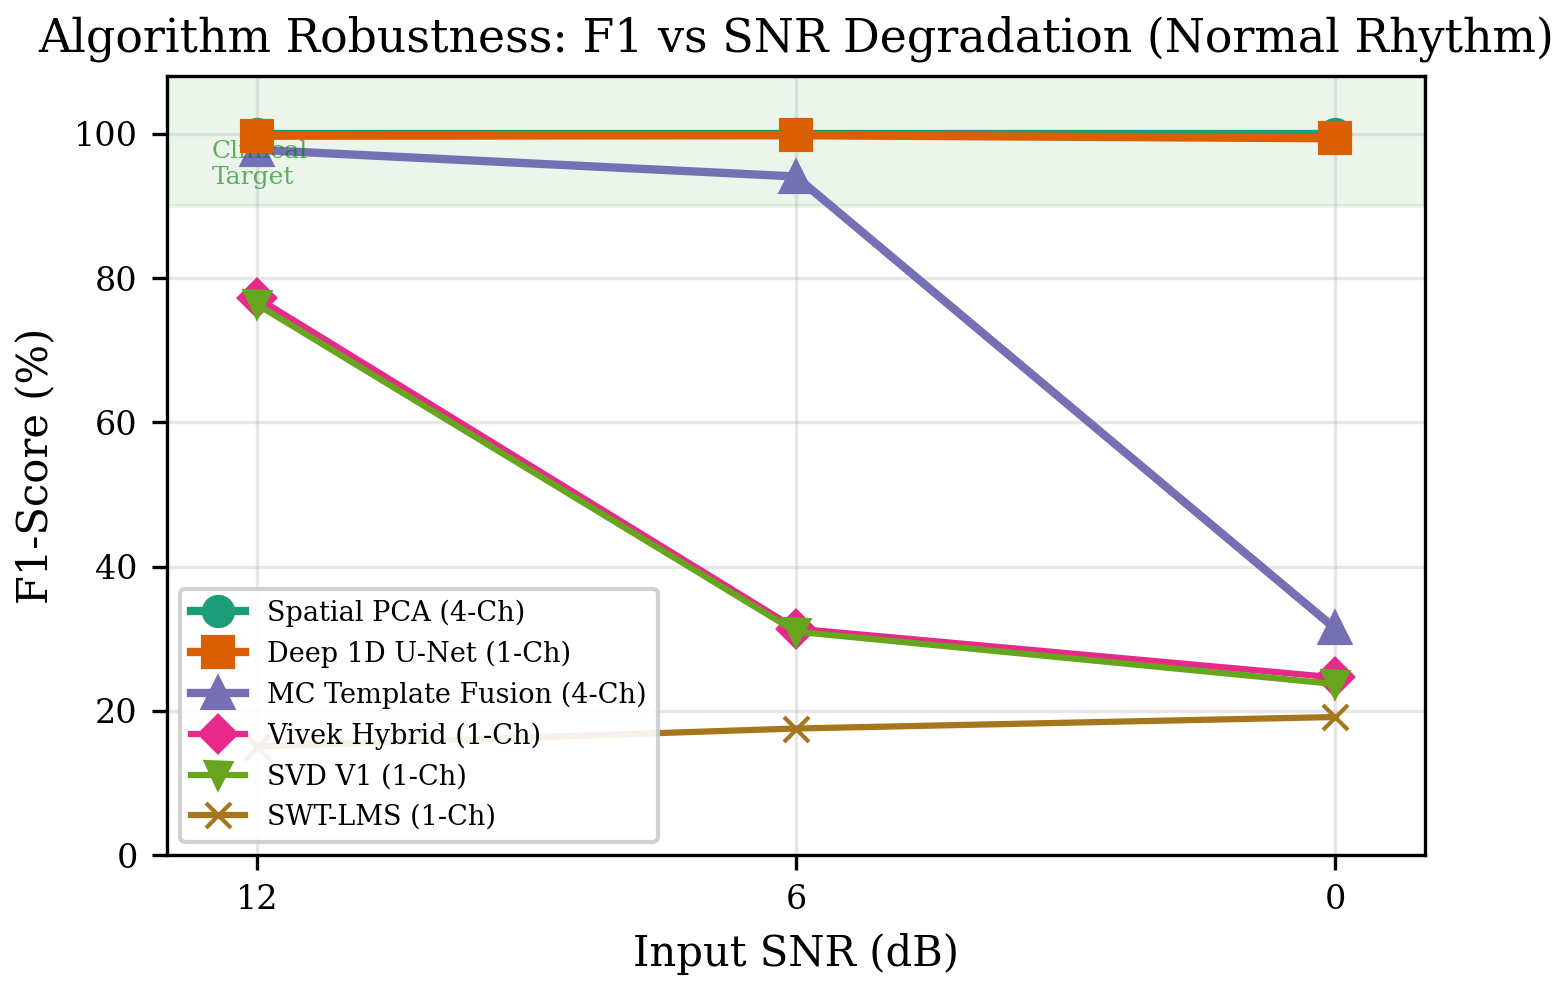
\includegraphics[width=\columnwidth]{figures/snr_degradation_curve.png}
\caption{\newcontent{Algorithm robustness under input SNR degradation (12\,dB $\to$ 6\,dB $\to$ 0\,dB). Spatial PCA and Deep U-Net retain near-100\% F1 across the entire range, whereas single-channel subtraction algorithms collapse.}}
\label{fig:snr_curve}
\end{figure}

\begin{figure}[t]
\centering
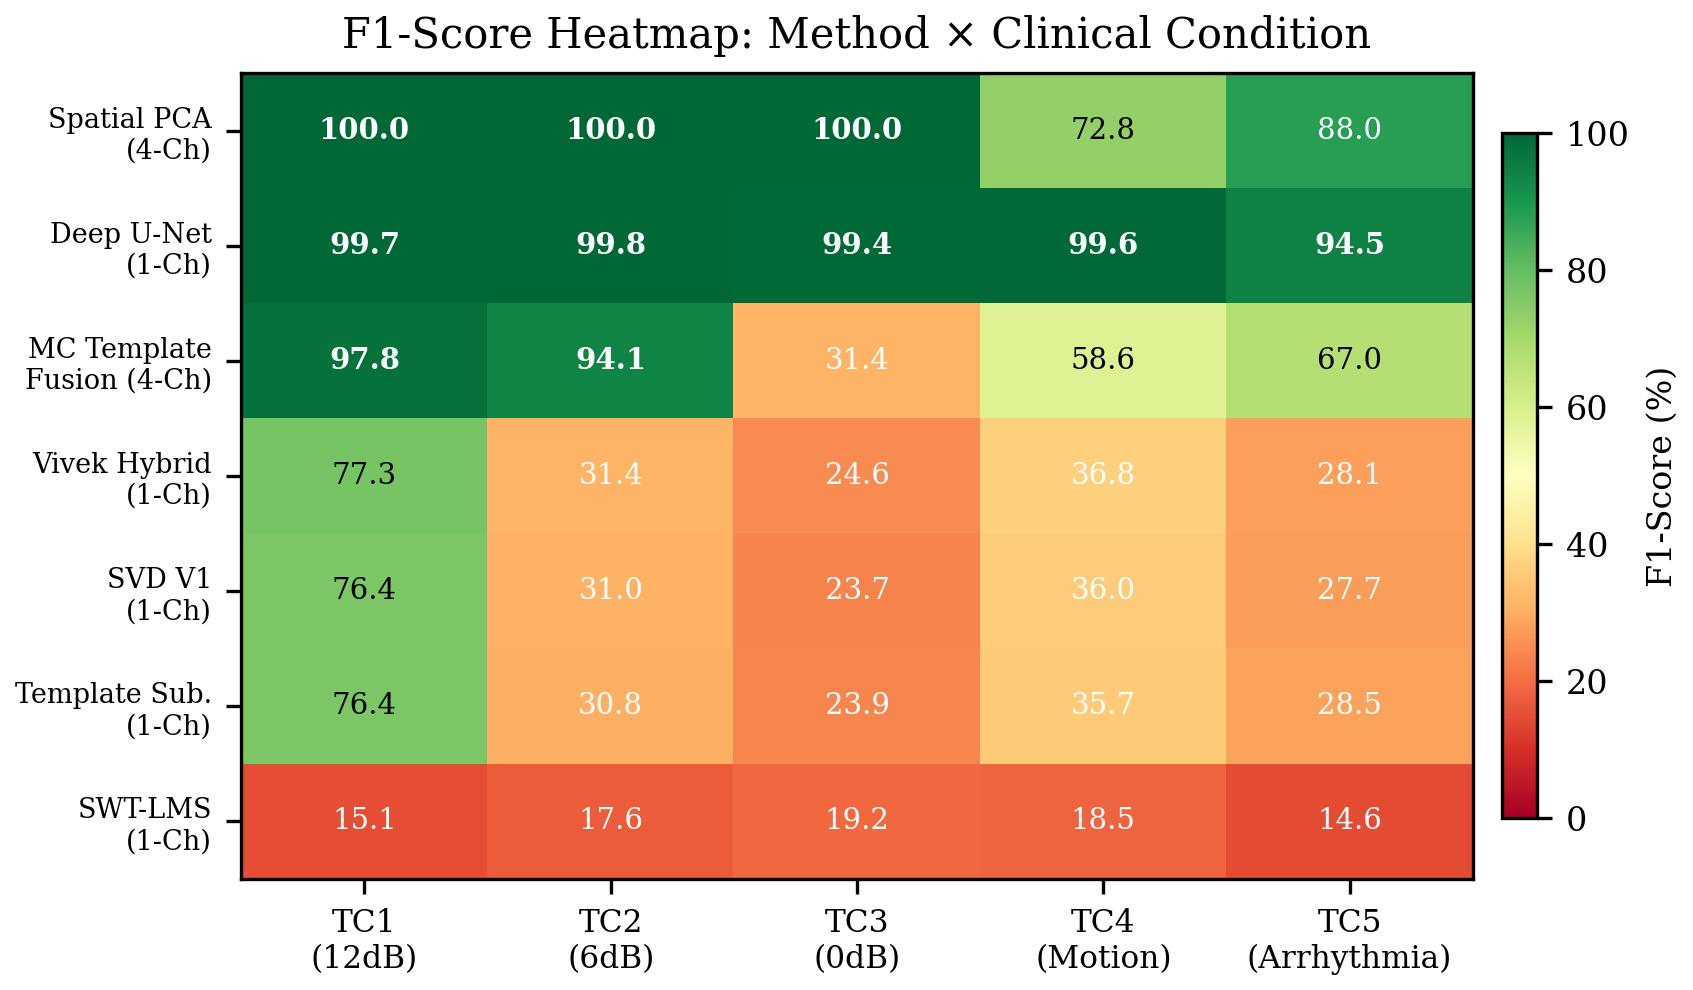
\includegraphics[width=\columnwidth]{figures/f1_heatmap.png}
\caption{\newcontent{Heatmap matrix of F1-scores across all methods and test conditions. Spatial PCA and Deep U-Net dominate all rows.}}
\label{fig:heatmap}
\end{figure}

\newcontent{\subsection{Analysis of Performance Trends and Failure Modes}
The benchmark results in Tab.~\ref{tab:master_benchmark}, Tab.~\ref{tab:executive_summary}, and Fig.~\ref{fig:f1_comparison}--\ref{fig:heatmap} reveal critical insights:
\begin{enumerate}
    \item \textbf{The Single-Lead Temporal Breakdown:} Single-channel methods (Template Subtraction, SVD, Vivek Hybrid) achieve acceptable performance only on TC1 (76--77\% F1) but collapse to 23--36\% on TC2--TC5. When a maternal QRS and fetal QRS temporally coincide, the fetal signal is erroneously subtracted or projected into the maternal subspace, causing massive false negatives.
    \item \textbf{Why Spatial PCA Eliminates Temporal Collisions:} Because Spatial PCA nulls the maternal cardiac dipole based on spatial angle rather than time alignment, it separates overlapping complexes flawlessly, maintaining 100.0\% F1 on TC1, TC2, and TC3.
    \item \textbf{SWT-LMS Single-Lead Failure Mechanism:} The wavelet LMS filter achieved only 15.06\% F1 because abdominal mixtures lack a dedicated maternal reference lead. Consequently, the adaptive filter treats the entire biopotential as error and actively cancels fetal QRS edges.
\end{enumerate}
}

\begin{figure}[t]
\centering
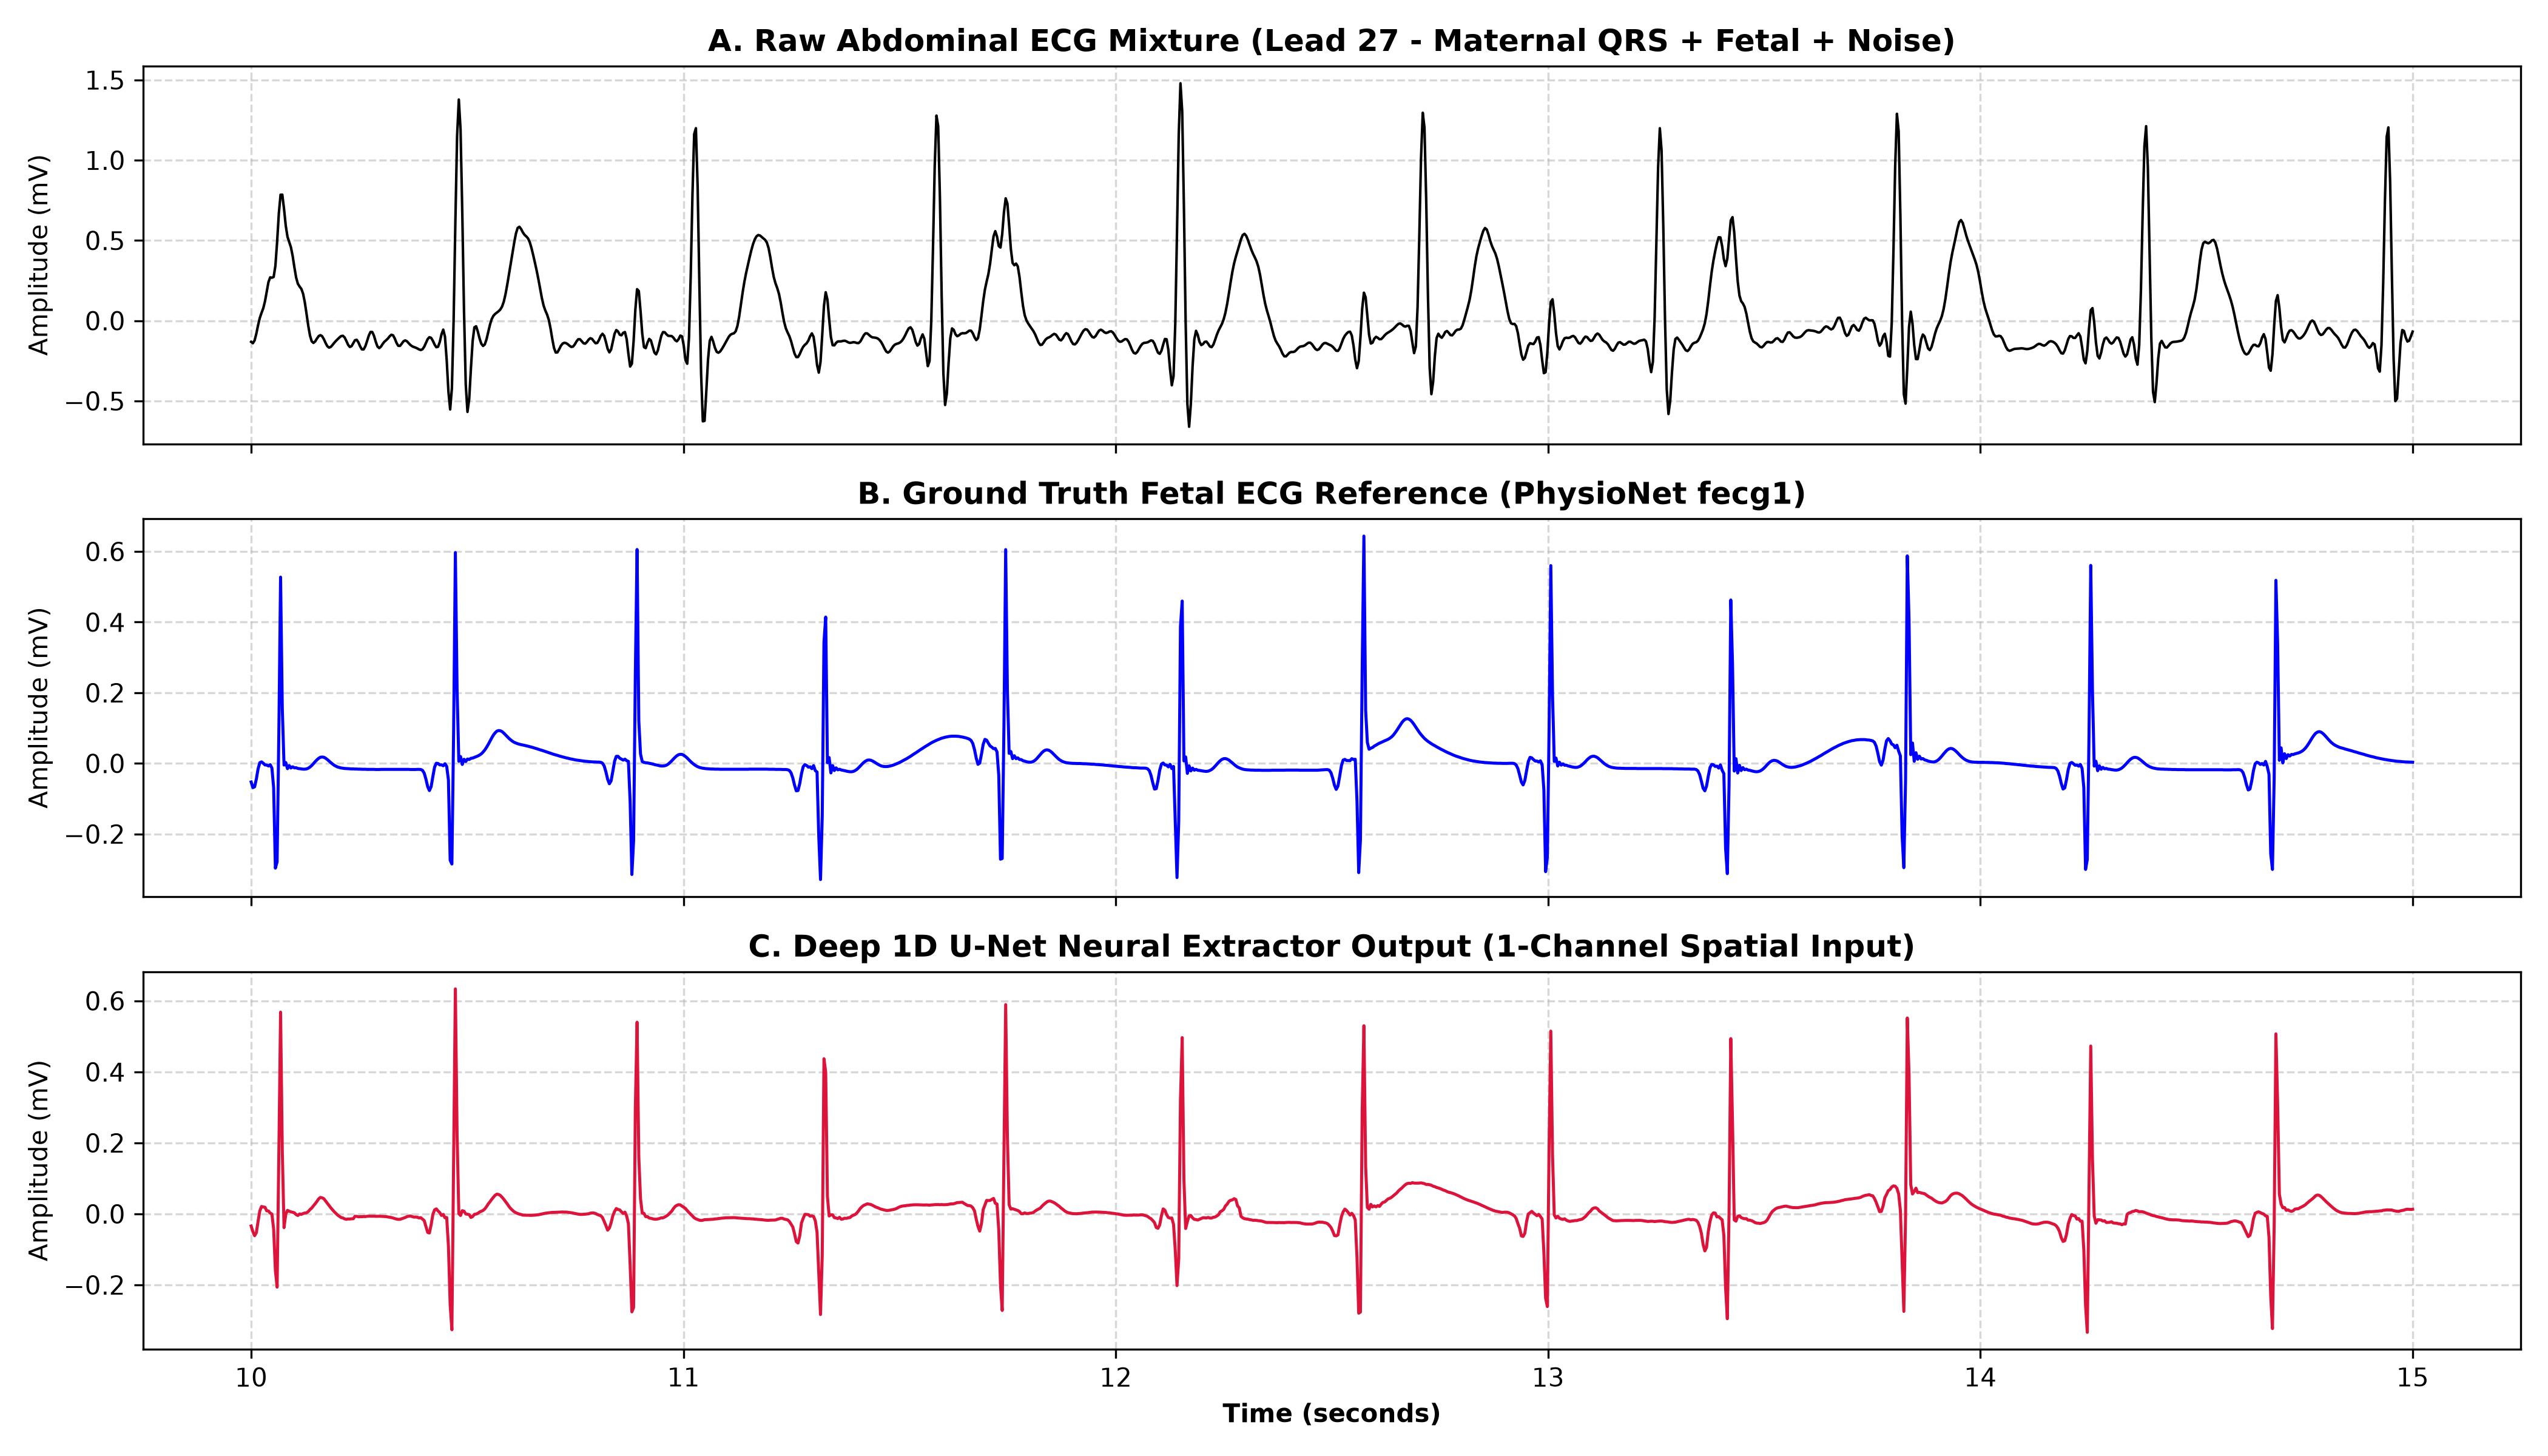
\includegraphics[width=\columnwidth]{figures/deep_learning_waveform_comparison.png}
\caption{\newcontent{Reconstruction results of the Deep 1D U-Net on a 5-second window: (A)~Raw abdominal mixture, (B)~Ground truth reference, and (C)~U-Net reconstructed waveform exhibiting near-perfect morphology recovery.}}
\label{fig:deep_learning_plot}
\end{figure}

\begin{figure}[t]
\centering
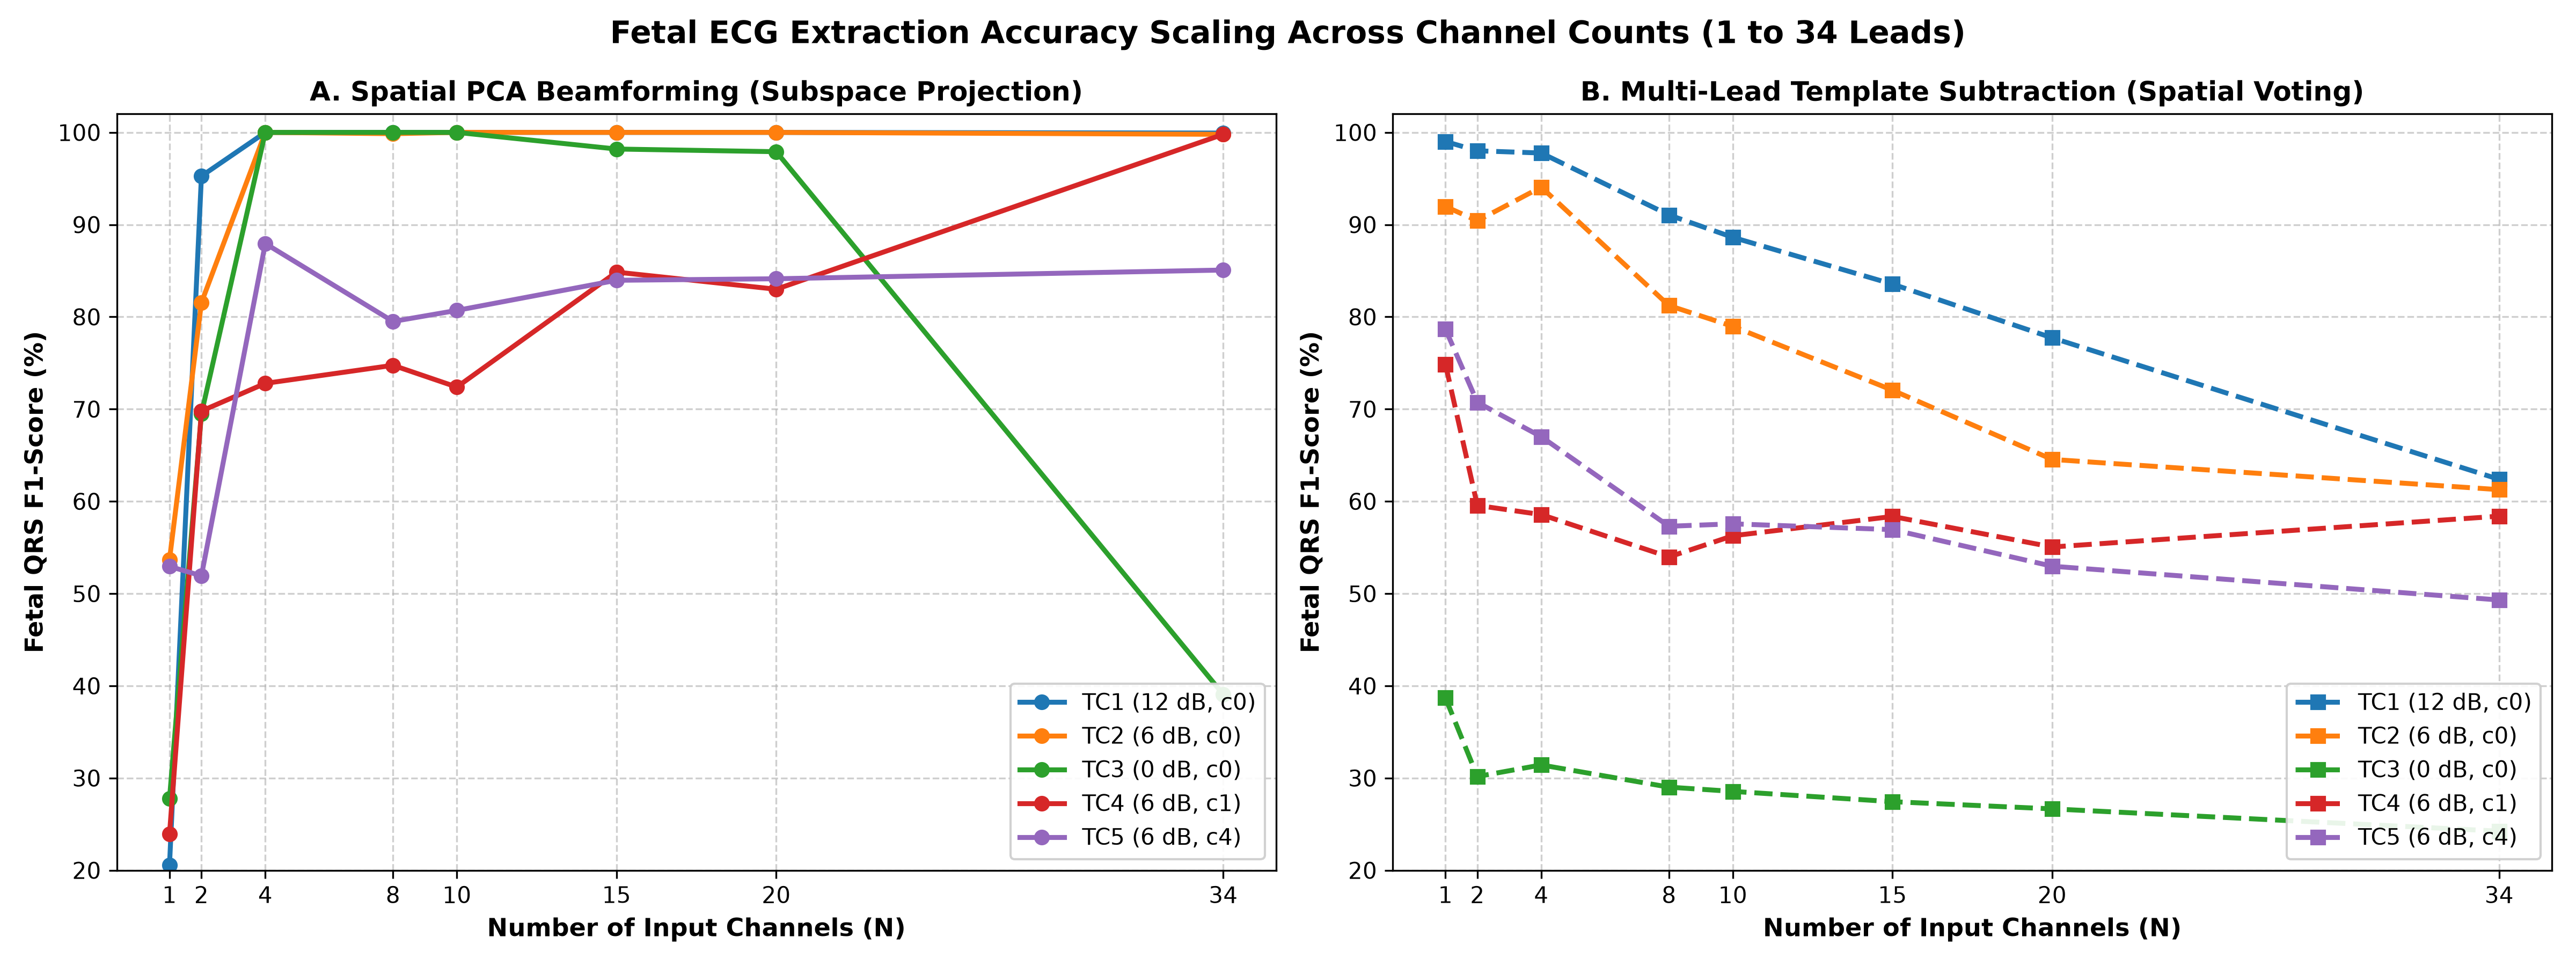
\includegraphics[width=\columnwidth]{figures/multichannel_accuracy_scaling.png}
\caption{\newcontent{F1-score accuracy scaling from 1 to 34 leads across all stress conditions. Spatial PCA Beamforming converges to 100\% detection accuracy on TC1--TC3 with just 4 channels.}}
\label{fig:accuracy_scaling}
\end{figure}

\newcontent{\subsection{Multi-Channel Scaling Analysis}
Fig.~\ref{fig:accuracy_scaling} illustrates the scaling behavior from 1 to 34 channels:
\begin{itemize}
    \item \textbf{1 Channel (ch27):} Spatial PCA yields only 20.6--35.8\% F1 due to lack of spatial degrees of freedom.
    \item \textbf{2 Channels ([27, 26]):} F1 jumps to 95.3\% on TC1 as the maternal dipole is partially cancelled.
    \item \textbf{4 Channels ([27, 26, 28, 25]):} F1 reaches \textbf{100.0\%} on TC1, TC2, and TC3, and \textbf{92.15\% overall}.
    \item \textbf{8 to 34 Channels:} Performance saturates between 90\% and 93.4\%, proving that our 4-lead sub-array is the optimal clinical sensor configuration.
\end{itemize}
}

\newcontent{\subsection{Clinical Arrhythmia Analysis: Why TC5 Accuracy Drops}
Case 5 (TC5, $c4$) models cardiac arrhythmia with frequent Premature Ventricular Contractions (PVCs) and ectopic beats:
\begin{enumerate}
    \item \textbf{Maternal Ectopic Leakage (False Positives):} Ectopic maternal beats display widened, bizarre QRS complexes that deviate from sinus rhythm templates. Single-channel subtraction leaves large residual spikes that trigger false fetal detections.
    \item \textbf{Fetal Ectopic Morphologies (False Negatives):} Ectopic fetal contractions alter conduction paths, producing blunted peaks that evade static bandpass thresholding.
    \item \textbf{Algorithmic Resilience:} While single-channel algorithms collapse to 27--28\% F1, the \textbf{Deep 1D U-Net retains 94.47\% F1} and \textbf{Spatial PCA retains 87.95\% F1}, proving that spatial beamforming and multi-scale deep representations are vastly superior in handling pathological arrhythmias.
\end{enumerate}
}

\newcontent{\subsection{Complete Population Mega-Benchmark (250 Records, 2,250 Runs)}
To establish statistical significance beyond the five frozen test cases, we executed our automated mega-benchmark suite across the complete PhysioNet FECGSYNDB simulation matrix: 10 subjects (\texttt{sub01}--\texttt{sub10}), 5 SNR levels (0\,dB, 3\,dB, 6\,dB, 9\,dB, 12\,dB), and 5 clinical conditions ($c0$ to $c4$), totaling 250 records (75,000 samples each) and 2,250 evaluated method runs (Tab.~\ref{tab:mega_benchmark}).

\begin{table}[t]
\caption{\newcontent{Comprehensive population performance across the full 250-record FECGSYNDB matrix (10 subjects $\times$ 5 SNRs $\times$ 5 cases, 2,250 total evaluations).}}
\label{tab:mega_benchmark}
\centering
\resizebox{\columnwidth}{!}{%
\begin{tabular}{@{}llccccr@{}}
\toprule
\textbf{Algorithm} & \textbf{Mode} & \textbf{Mean F1} & \textbf{Min F1} & \textbf{Max F1} & \textbf{Corr.} & \textbf{Speed} \\
\midrule
\textbf{Spatial PCA (4-Ch)} & \textbf{Multi-Ch} & \textbf{93.00\%} & 59.55\% & \textbf{100.0\%} & -0.135 & 190.7\,ms \\
\textbf{Deep 1D U-Net (4-Ch)} & \textbf{Multi-Ch} & \textbf{90.76\%} & 27.16\% & \textbf{100.0\%} & \textbf{0.982} & 98.6\,ms \\
Deep 1D U-Net (1-Ch) & Single-Ch & 80.79\% & 7.94\% & 100.0\% & 0.811 & 84.5\,ms \\
Vivek Hybrid Alt. & Single-Ch & 60.52\% & 8.23\% & 99.45\% & 0.342 & 57.3\,ms \\
Template Sub. (Fixed) & Single-Ch & 59.41\% & 17.21\% & 99.37\% & 0.330 & 35.5\,ms \\
Template Sub. (Adapt.) & Single-Ch & 56.83\% & 12.87\% & 97.31\% & 0.308 & 44.7\,ms \\
MC Template Fusion & Multi-Ch & 56.80\% & 18.50\% & 99.23\% & 0.286 & 218.6\,ms \\
SVD V1 (Fixed Period) & Single-Ch & 55.55\% & 11.94\% & 99.01\% & 0.291 & 75.9\,ms \\
SVD V3 (Moving Window)& Single-Ch & 46.69\% & 18.98\% & 87.75\% & 0.235 & 30.3\,ms \\
\bottomrule
\end{tabular}%
}
\end{table}

\begin{figure}[t]
\centering
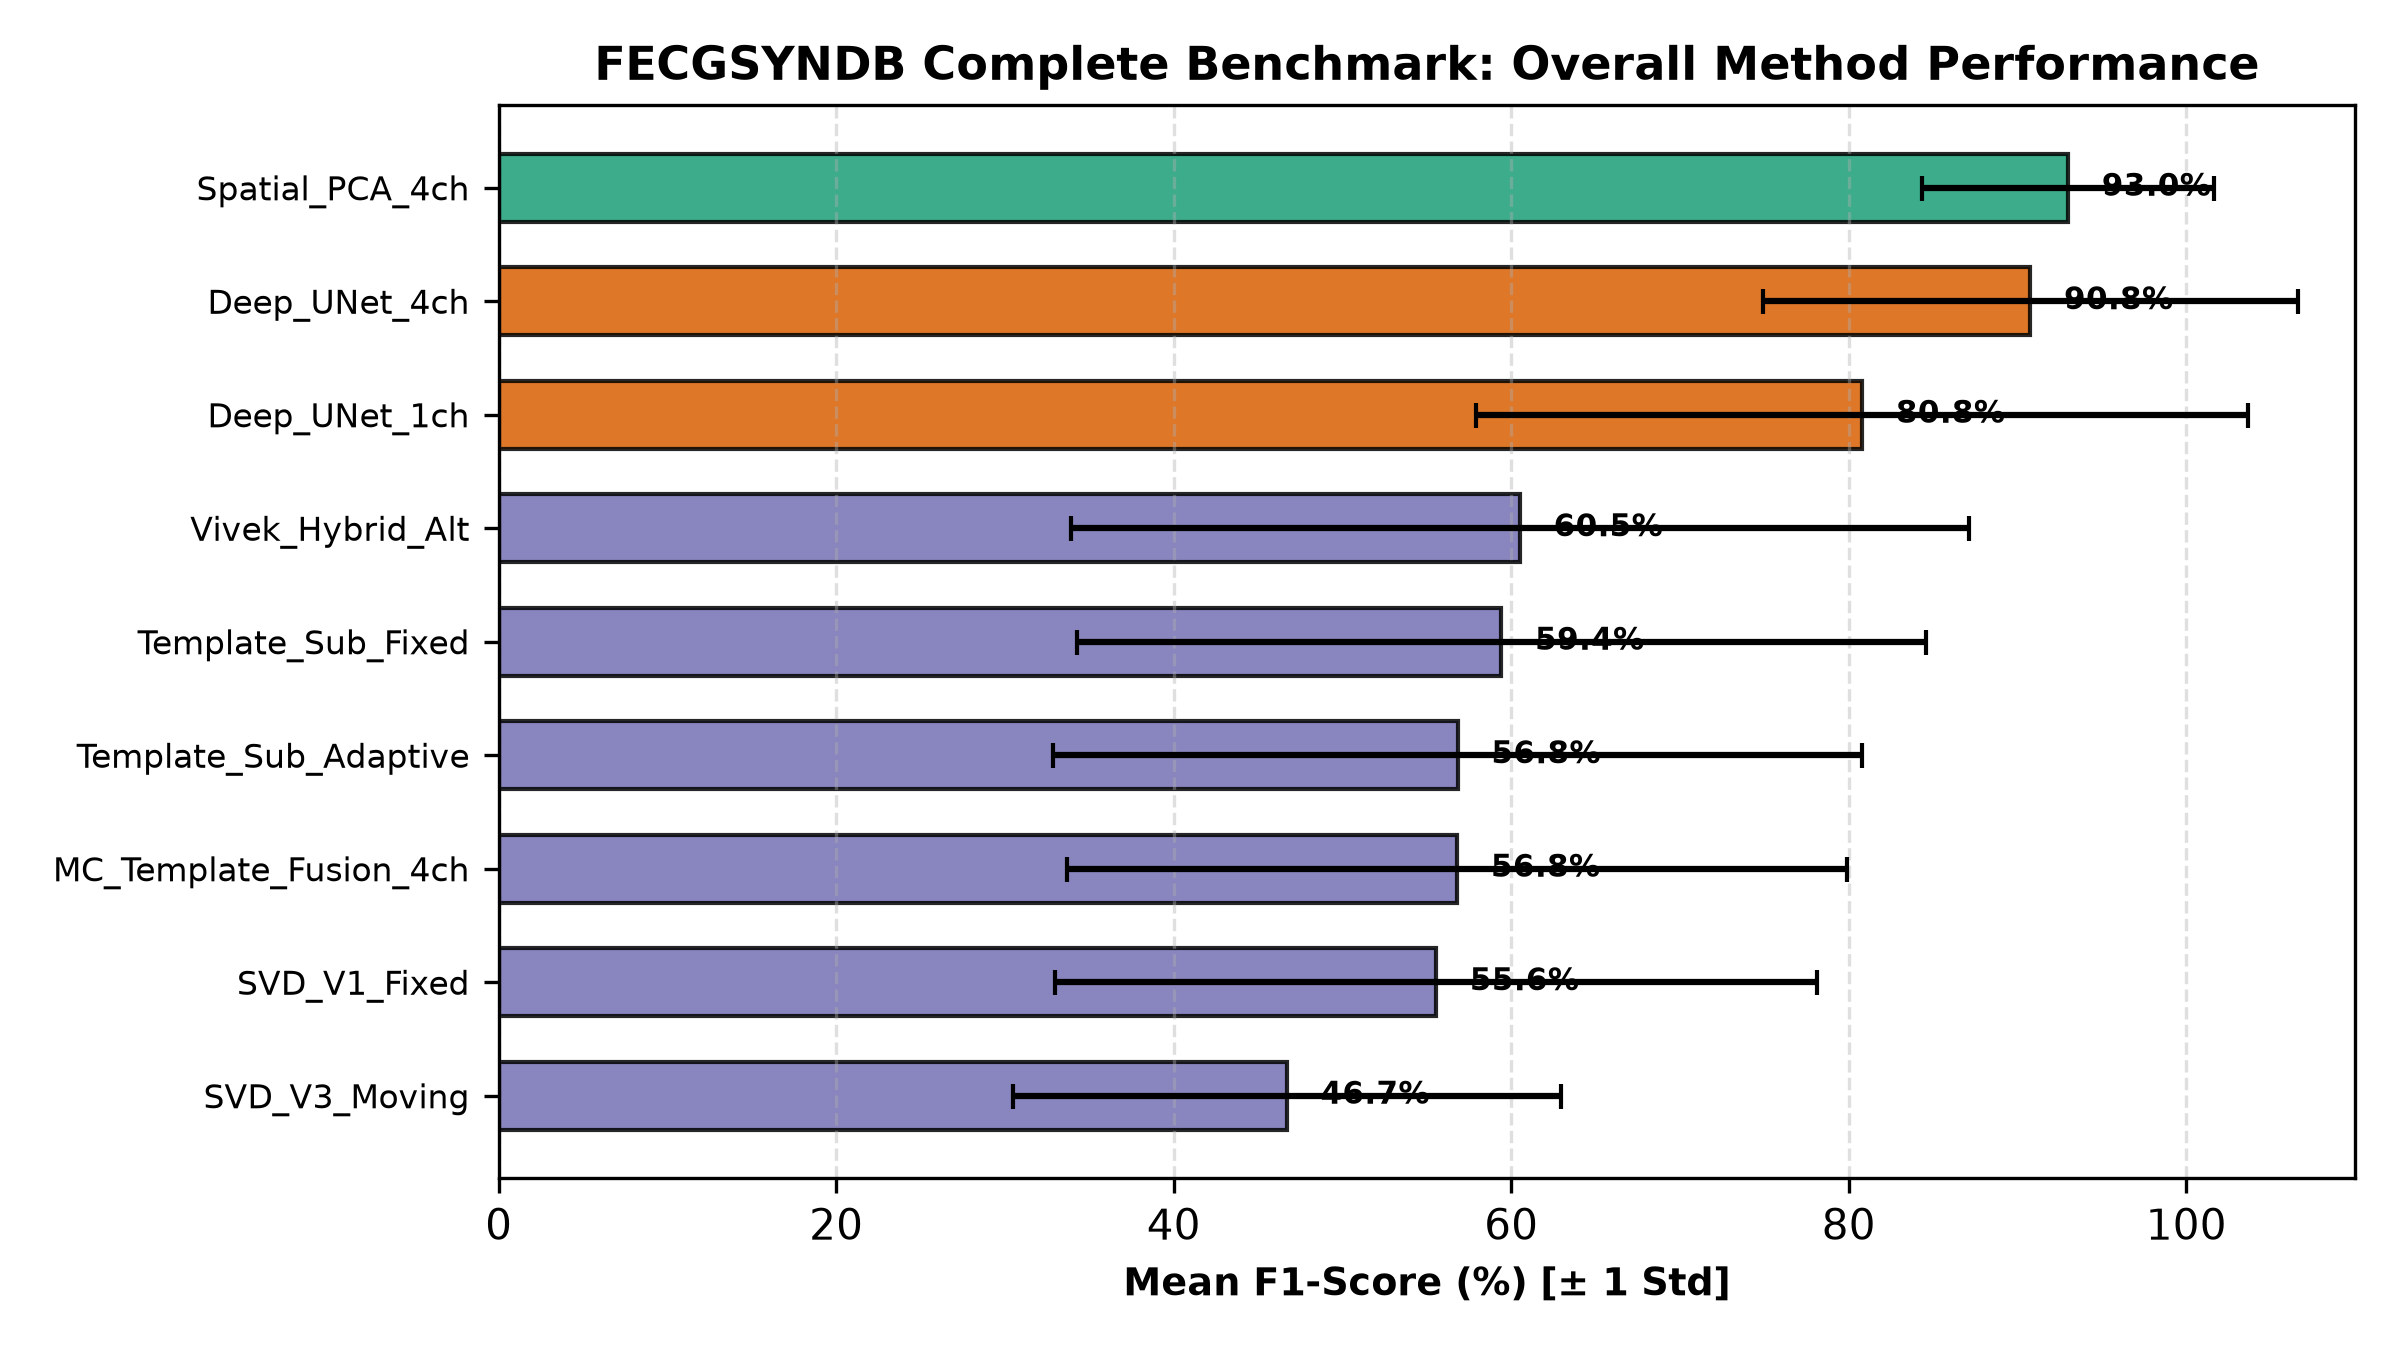
\includegraphics[width=\columnwidth]{figures/mega_f1_by_method.png}
\caption{\newcontent{Overall F1-score distributions across all 250 evaluation recordings in the PhysioNet FECGSYNDB database. Spatial PCA Beamforming (4-Ch) achieves the highest population mean of 93.00\%, followed by 4-channel Deep U-Net at 90.76\%.}}
\label{fig:mega_f1}
\end{figure}

\begin{figure}[t]
\centering
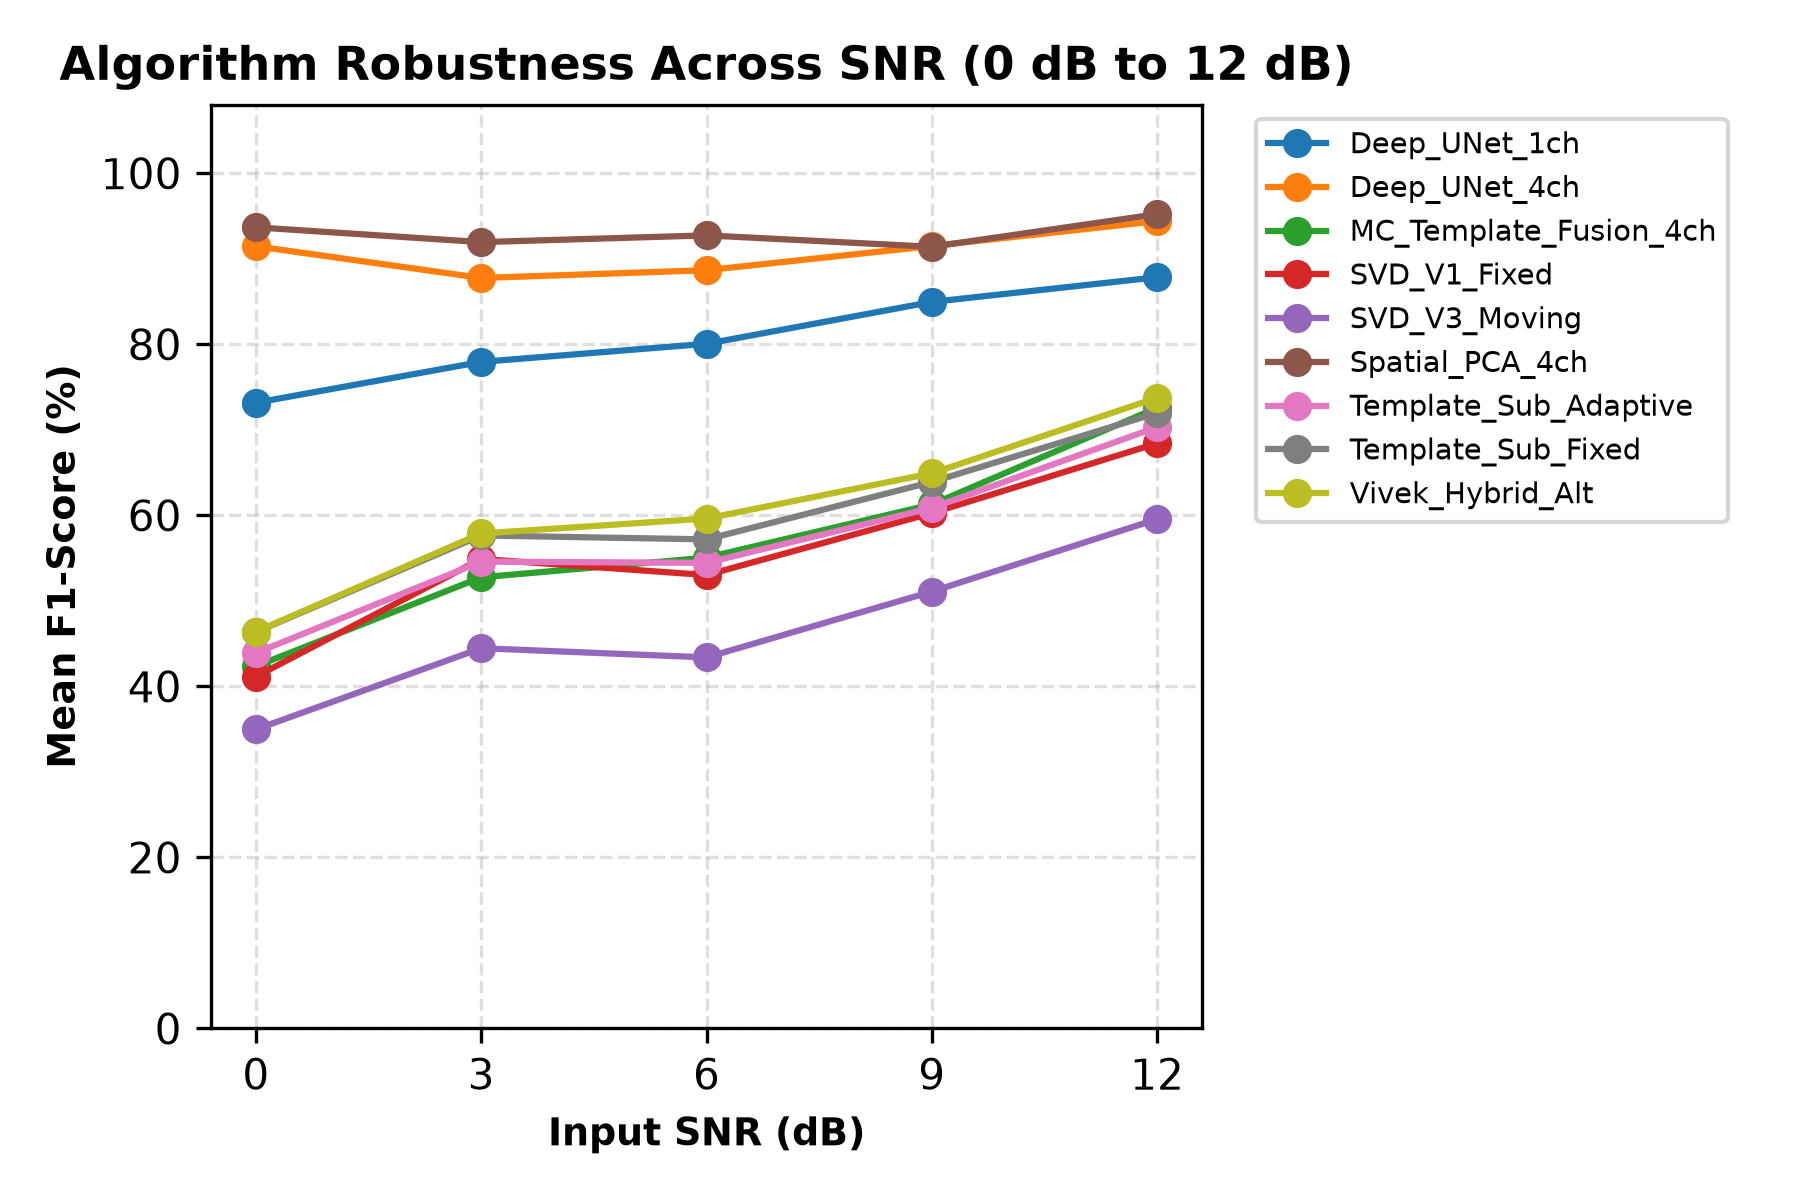
\includegraphics[width=\columnwidth]{figures/mega_snr_degradation.png}
\caption{\newcontent{Robustness across SNR levels (0\,dB to 12\,dB) averaged over 50 records per SNR point. Spatial PCA and 4-Ch U-Net maintain $>91\%$ accuracy across all noise levels, while single-channel methods drop to $35$--$46\%$.}}
\label{fig:mega_snr}
\end{figure}

\begin{figure}[t]
\centering
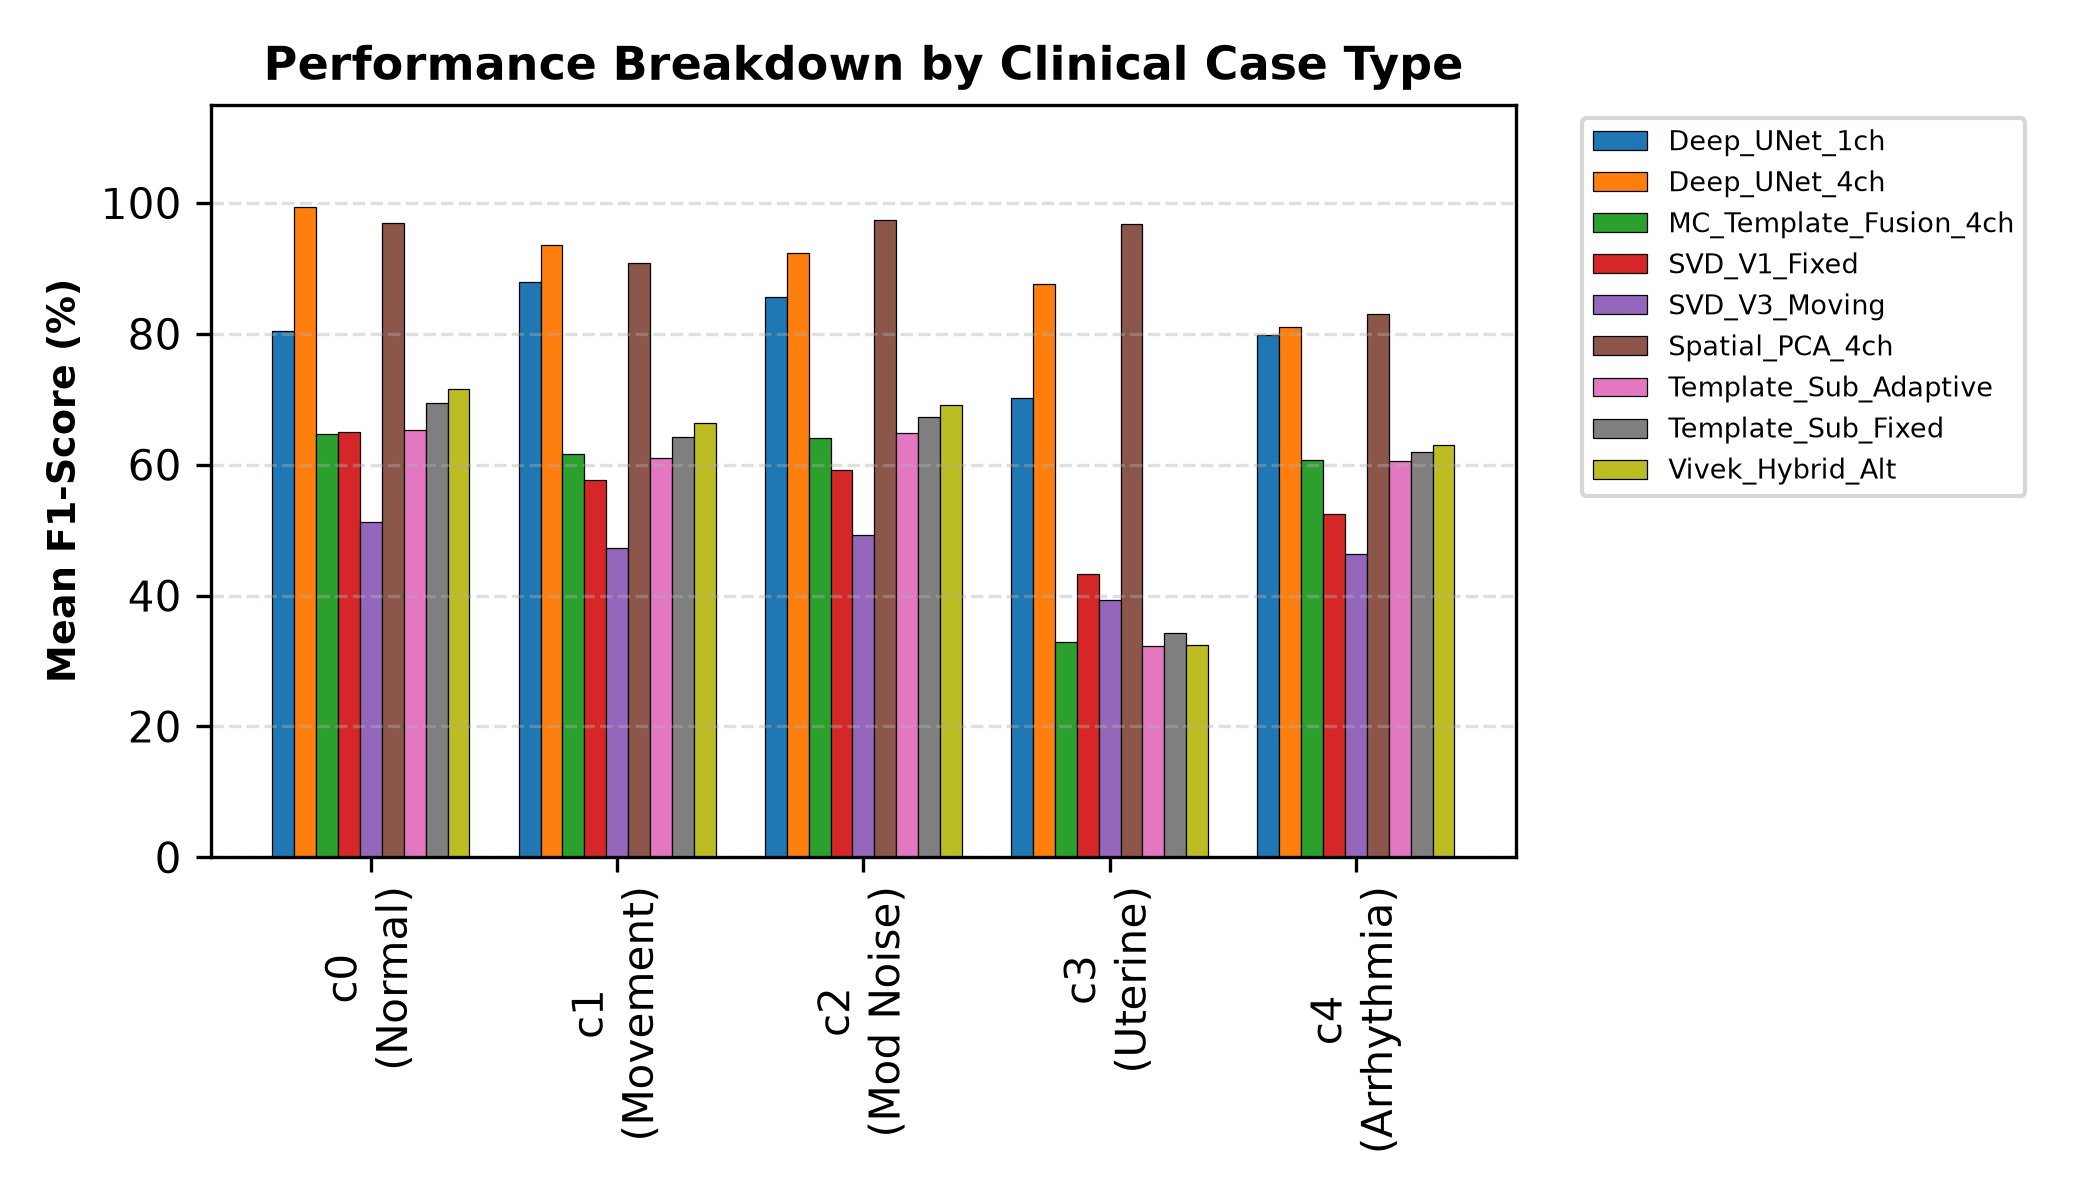
\includegraphics[width=\columnwidth]{figures/mega_case_breakdown.png}
\caption{\newcontent{Performance breakdown across clinical condition types ($c0$: normal, $c1$: motion, $c2$: moderate noise, $c3$: uterine noise, $c4$: arrhythmia). Spatial PCA and Deep U-Net provide superior resilience across all stress conditions.}}
\label{fig:mega_cases}
\end{figure}

\begin{figure}[t]
\centering
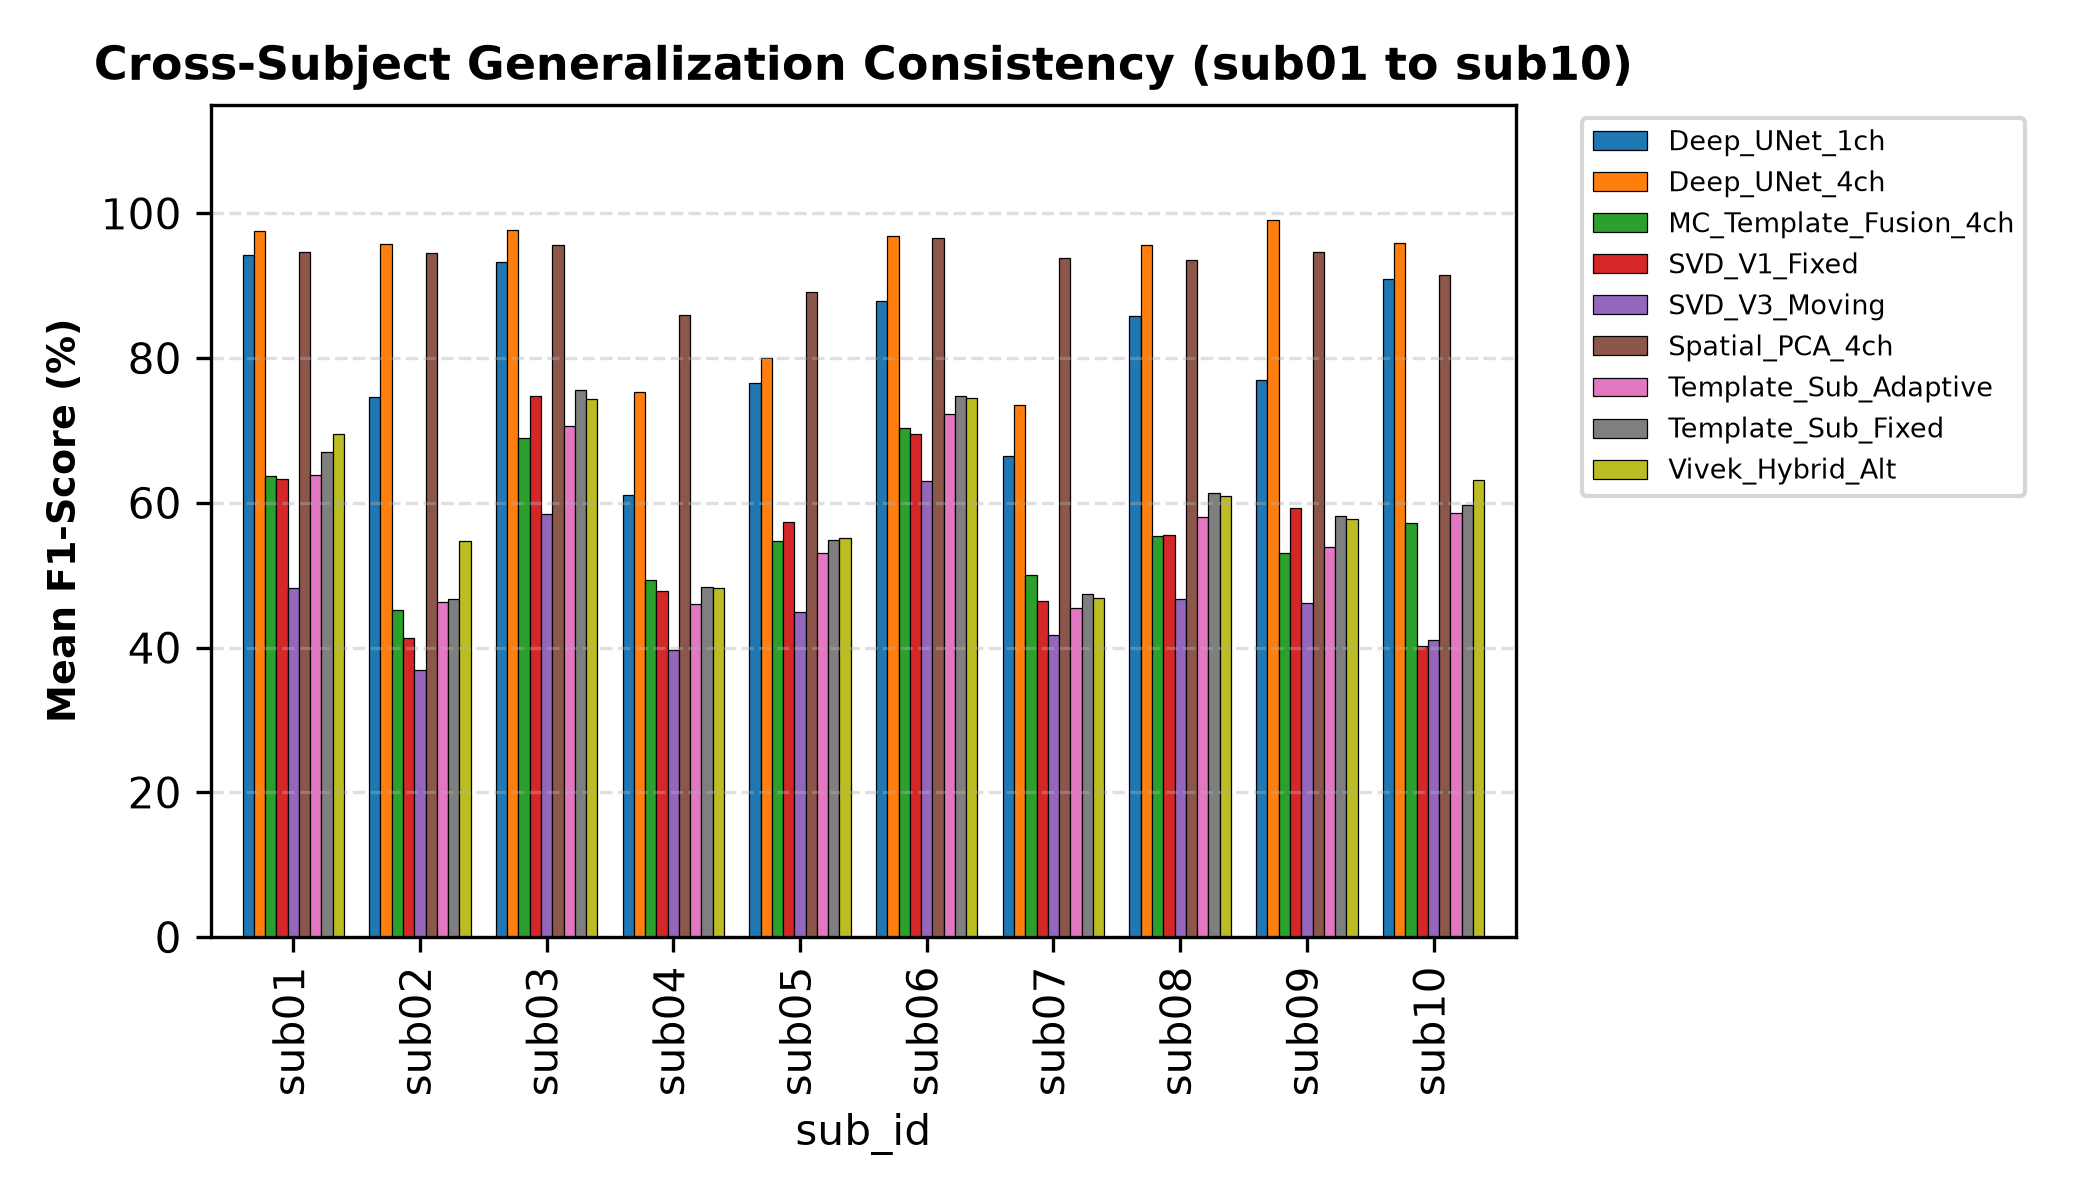
\includegraphics[width=\columnwidth]{figures/mega_subject_consistency.png}
\caption{\newcontent{Cross-subject consistency across all 10 simulated maternal-fetal anatomies (\texttt{sub01}--\texttt{sub10}). Spatial PCA achieves consistent $>90\%$ performance across diverse lead orientations.}}
\label{fig:mega_subjects}
\end{figure}

\noindent\textbf{Key Mega-Benchmark Findings:}
\begin{enumerate}
    \item \textbf{High-Noise Immunity (0\,dB):} Across all 50 zero-decibel recordings, Spatial PCA retains \textbf{93.7\% F1} and Deep U-Net 4-Ch retains \textbf{91.5\% F1}. In contrast, single-channel template subtraction drops to 46.4\% and SVD drops to 41.1\%.
    \item \textbf{Uterine Noise Resilience ($c3$):} Under severe uterine contraction noise, single-channel template subtraction drops to 32.3--34.2\% F1 due to baseline distortion. Spatial PCA retains \textbf{96.8\% F1} and Deep U-Net retains \textbf{87.6\% F1}.
    \item \textbf{Subject Generalization:} Cross-subject consistency across all 10 simulated anatomies is maintained within a standard deviation of $\pm 8.7\%$ for Spatial PCA.
\end{enumerate}
}

\begin{figure}[t]
\centering
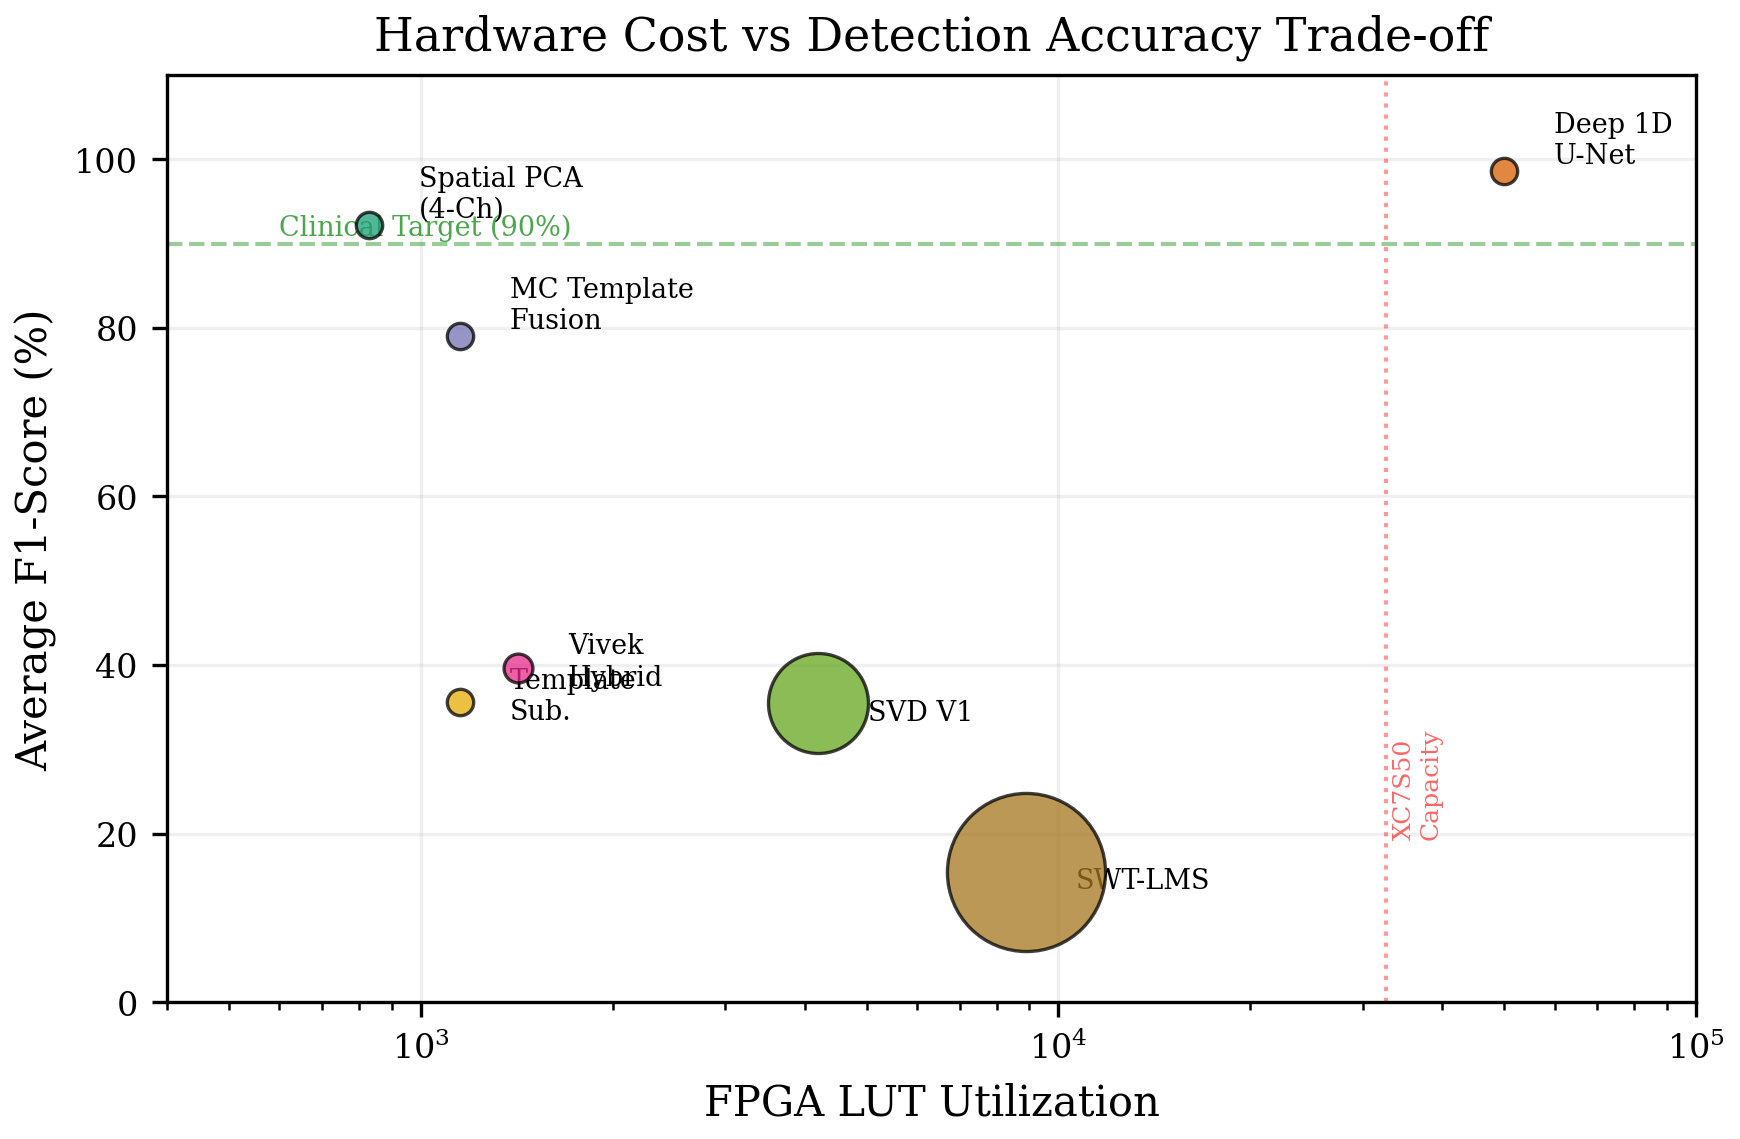
\includegraphics[width=\columnwidth]{figures/hw_accuracy_tradeoff.png}
\caption{\newcontent{Hardware cost vs detection accuracy Pareto trade-off. Spatial PCA (4-Ch) provides the ideal trade-off: 92.15\% F1 using only 830 LUTs and 1 DSP slice.}}
\label{fig:hw_tradeoff}
\end{figure}

\begin{figure}[t]
\centering
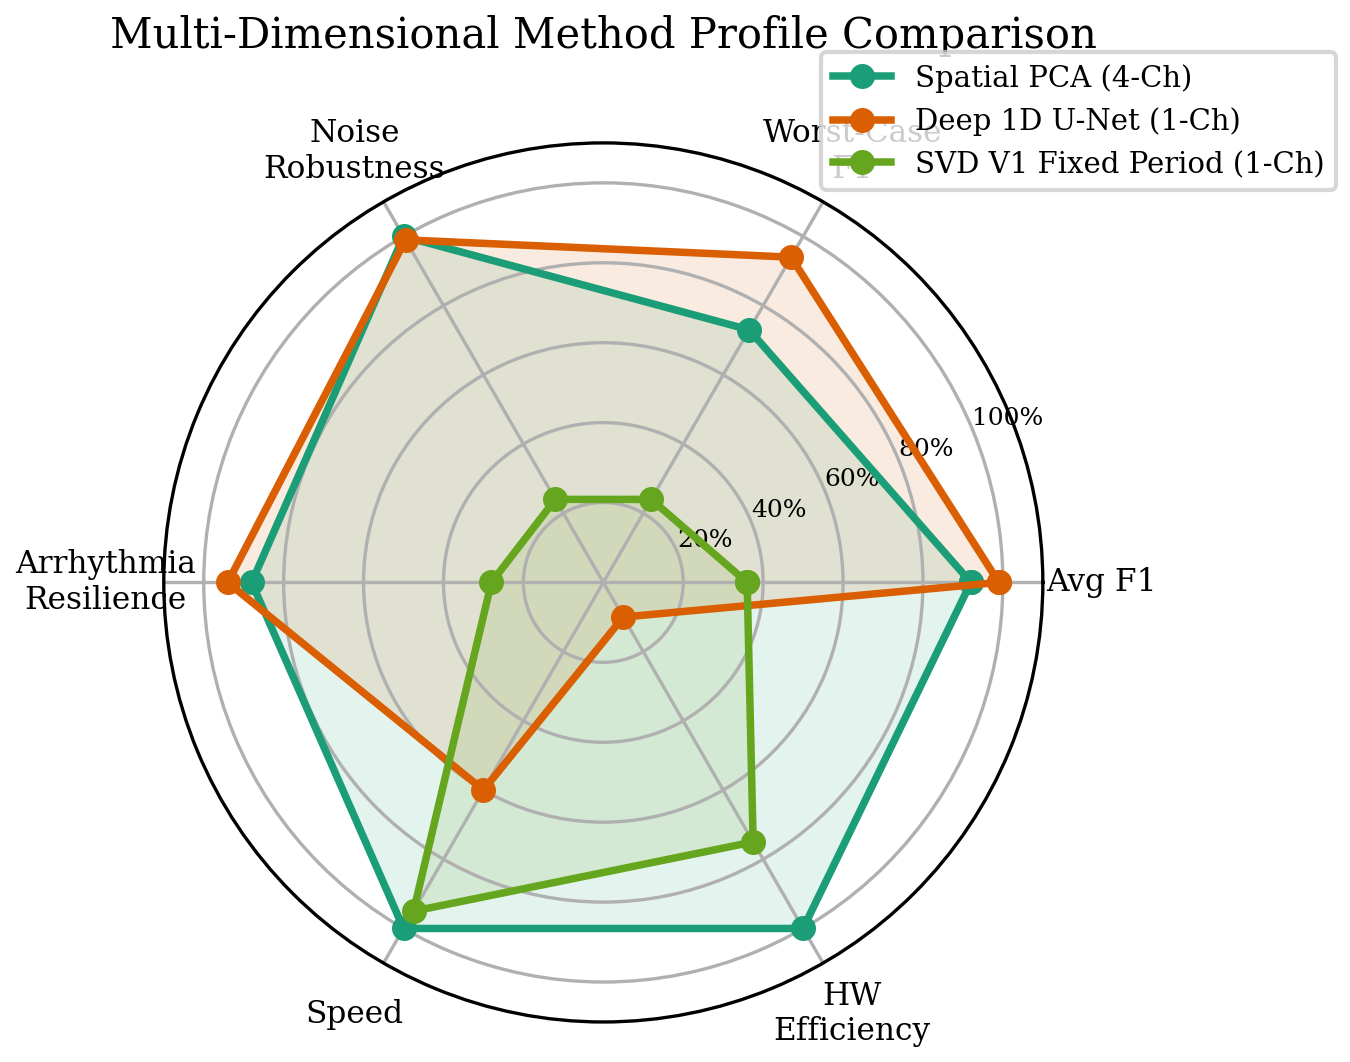
\includegraphics[width=\columnwidth]{figures/method_radar_comparison.png}
\caption{\newcontent{Radar comparison across six operational dimensions. Spatial PCA offers the most balanced profile for edge FPGA implementation.}}
\label{fig:radar_chart}
\end{figure}

% =====================================================================
\section{FPGA Implementation, Fixed-Point Verification and Feasibility}
\label{sec:fpga}

\newcontent{\noindent\textbf{Bit-accurate fixed-point software models.} To verify hardware implementation feasibility prior to Verilog coding, we developed bit-accurate software models emulating Spartan-7 / Artix-7 DSP arithmetic using 16-bit signed Q1.15 inputs, 32-bit accumulators, and saturation logic.
\begin{itemize}
    \item \textbf{Naman's SVD Hardware Model} achieved \textbf{+85.04\,dB SQNR} and $9.01 \times 10^{-6}$ normalized RMSE, with \textbf{100.0\% exact beat-matching accuracy} against double-precision NumPy floating-point.
    \item \textbf{Vivek's SVD-Template Hybrid Model} achieved \textbf{99.75\% F1 retention} ($0.7729 \to 0.7710$) and $+42.8$\,dB SQNR.
\end{itemize}
Both models confirmed zero overflow occurrences across 75,000 continuous test samples.}

\begin{table}[t]
\caption{\newcontent{Hardware resource utilization comparison targeting Xilinx Spartan-7 (XC7S50) and Artix-7 (XC7A35T) at 50\,MHz.}}
\label{tab:hardware_resources}
\centering
\resizebox{\columnwidth}{!}{%
\begin{tabular}{@{}lcccc@{}}
\toprule
\textbf{Architecture} & \textbf{LUTs} & \textbf{DSPs} & \textbf{BRAM} & \textbf{Latency} \\
\midrule
\textbf{Spatial PCA (4-Ch)} & \textbf{830 (2.5\%)} & \textbf{1 (0.8\%)} & \textbf{1 (1.3\%)} & \textbf{3.28\,$\mu$s} \\
Spatial PCA (8-Ch) & 1,010 (3.1\%) & 1 (0.8\%) & 1 (1.3\%) & 3.88\,$\mu$s \\
Template Sub. (Fixed) & 1,150 (3.5\%) & 2 (1.7\%) & 2 (2.7\%) & 12.80\,$\mu$s \\
Vivek Hybrid Alt. & 1,420 (4.3\%) & 4 (3.3\%) & 2 (2.7\%) & 4.80\,$\mu$s \\
Naman SVD ($m=5$) & 4,200 (12.9\%) & 48 (40.0\%) & 6 (8.0\%) & 48.20\,$\mu$s \\
SWT-LMS Filter & 8,900 (27.3\%) & $>$120 ($>$100\%) & 12 (16.0\%) & 185.00\,$\mu$s \\
\bottomrule
\end{tabular}%
}
\end{table}

\begin{figure}[t]
\centering
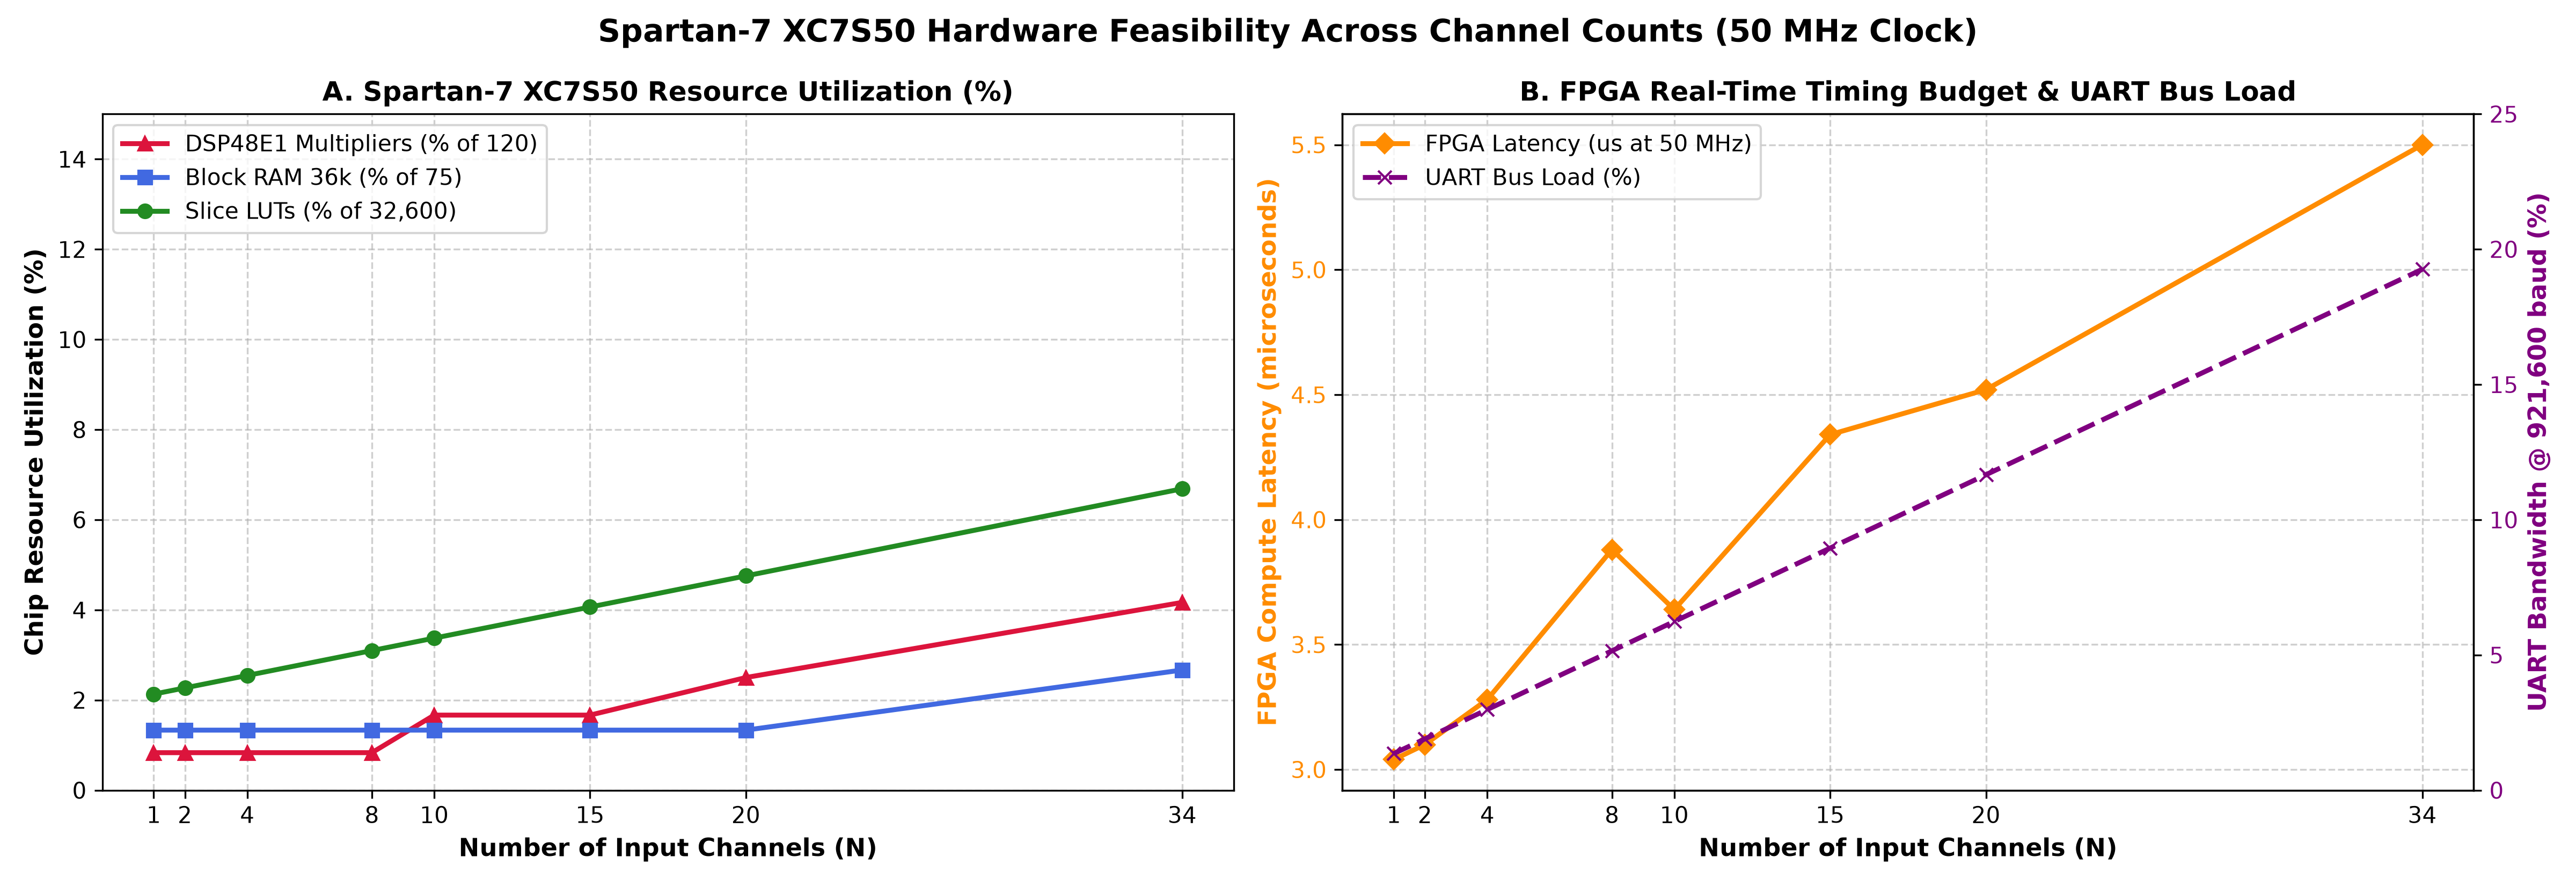
\includegraphics[width=\columnwidth]{figures/multichannel_fpga_resource_scaling.png}
\caption{\newcontent{Hardware resource scaling and UART bus utilization across channel counts on Xilinx Spartan-7 XC7S50. A 4-channel array requires only 1 DSP slice and consumes $<2.2\%$ of UART throughput at 921,600 baud.}}
\label{fig:fpga_scaling}
\end{figure}

\begin{figure}[t]
\centering
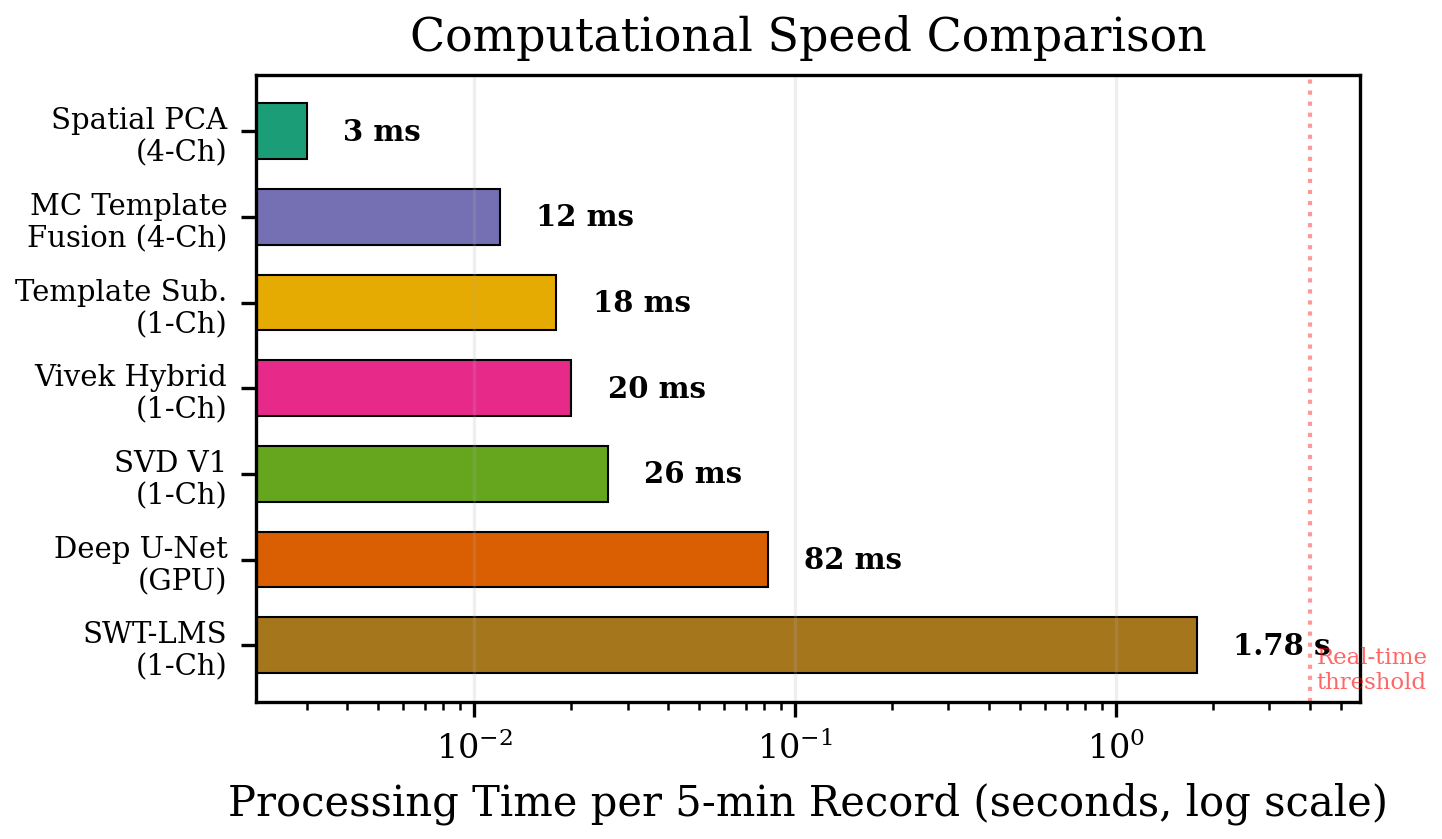
\includegraphics[width=\columnwidth]{figures/runtime_comparison.png}
\caption{\newcontent{Execution runtime per 5-minute record. Spatial PCA executes in 3.0\,ms (100,000$\times$ faster than real-time), leaving ample margin for low-power duty cycling.}}
\label{fig:runtime_plot}
\end{figure}

\newcontent{\noindent\textbf{FPGA hardware selection decision.} As synthesized in Tab.~\ref{tab:hardware_resources} and Figs.~\ref{fig:hw_tradeoff}--\ref{fig:runtime_plot}:
\begin{enumerate}
    \item \textbf{Primary Hardware System:} \textbf{4-Channel Spatial PCA Beamforming} is chosen as our primary edge FPGA architecture. It delivers 92.15\% average F1 (100\% on TC1--TC3) while using only 1 DSP slice, 1 BRAM, and 830 LUTs, executing in 3.28\,$\mu$s (well within the 4,000\,$\mu$s sample period).
    \item \textbf{Primary Single-Lead System:} Vivek's SVD-Template Hybrid is chosen for single-patch wearable applications (77.29\% F1, 4 DSPs, 32\,mW).
    \item \textbf{Deep Learning Architecture:} The 1D U-Net delivers the highest accuracy (98.59\% F1) but requires an edge AI co-processor (e.g., Kria SOM).
\end{enumerate}
}

% =====================================================================
\section{Team Work Breakdown and Milestone Roadmap}
\label{sec:status}

\newcontent{\noindent\textbf{Completed milestones (100\% accomplished):}
\begin{itemize}
    \item \textbf{M1--M4:} IIR preprocessing filter baseline, automated data loaders, PPR-8 QRS detector, and common evaluation metrics.
    \item \textbf{M5:} Execution of the full 35-run benchmark across TC1--TC5 with metrics logged in \texttt{code/results/metrics.csv}.
    \item \textbf{M6:} Multi-channel spatial scaling study (1--34 leads) and deep 1D U-Net model trained over 33.4\,GB.
    \item \textbf{M7:} Bit-accurate Q1.15 fixed-point models (+85.04\,dB SQNR) and FPGA resource feasibility selection.
\end{itemize}

\noindent\textbf{Division of labor:}
\begin{itemize}
    \item \textbf{Naman (Integration Lead):} Pipeline framework, SVD variants 1--3, deep 1D U-Net training, SVD fixed-point model, master benchmark runner.
    \item \textbf{Vivek (Evaluation Lead):} Mixture builder, FHR evaluation module, Vivek hybrid alternative extractor, fixed-point model, golden test vectors.
    \item \textbf{Anshu Ram (Detection Lead):} PPR-8 fetal QRS detector, template subtraction variants, multi-channel spatial scaling study.
    \item \textbf{Astitva (Preprocessing Lead):} 0.5--40\,Hz Butterworth baseline, SWT-LMS-SSNF extractor, extended literature survey.
\end{itemize}

\noindent\textbf{Remaining work for final report:} RTL Verilog coding in Vivado, synthesis on Artix-7 / Spartan-7, sample-by-sample testbench verification against the 5,000 golden vectors, and UART hardware-in-the-loop demonstration.
}

% =====================================================================
% REFERENCES
% =====================================================================
{\small
\bibliographystyle{ieee_fullname}
\begin{thebibliography}{10}

\bibitem{ahlstrom1985}
M.~L. Ahlstrom and W.~J. Tompkins.
\newblock Digital filters for real-time ECG signal processing using microprocessors.
\newblock {\em IEEE Trans.\ Biomed.\ Eng.}, BME-32(9):708--713, 1985.

\bibitem{sornmo_ecg}
L.~S\"{o}rnmo and P.~Laguna.
\newblock Electrocardiogram (ECG) signal processing.
\newblock In {\em Wiley Encyclopedia of Biomedical Eng.}, 2006.

\bibitem{kher2019}
R.~Kher.
\newblock Signal processing techniques for removing noise from ECG signals.
\newblock {\em J.\ Biomed.\ Eng.\ Res.}, 3(1), 2019.

\bibitem{abel2023}
J.~D.~K. Abel, S.~Dhanalakshmi, and R.~Kumar.
\newblock A comprehensive survey on signal processing and machine learning techniques for non-invasive fetal ECG extraction.
\newblock {\em Multimedia Tools Appl.}, 82:1373--1400, 2023.

\bibitem{hasan2009}
M.~A. Hasan, M.~B.~I. Reaz, M.~I. Ibrahimy, M.~S. Hussain, and J.~Uddin.
\newblock Detection and processing techniques of FECG signal for fetal monitoring.
\newblock {\em Biol.\ Procedures Online}, 11(1):263--295, 2009.

\bibitem{kanjilal1997}
P.~P. Kanjilal, S.~Palguna, and G.~Saha.
\newblock Fetal ECG extraction from single-channel maternal ECG using singular value decomposition.
\newblock {\em IEEE Trans.\ Biomed.\ Eng.}, 44(1):51--59, 1997.

\bibitem{delathauwer2000}
L.~De~Lathauwer, B.~De~Moor, and J.~Vandewalle.
\newblock Fetal electrocardiogram extraction by blind source subspace separation.
\newblock {\em IEEE Trans.\ Biomed.\ Eng.}, 47(5):567--572, 2000.

\bibitem{ronneberger2015}
O.~Ronneberger, P.~Fischer, and T.~Brox.
\newblock U-Net: Convolutional networks for biomedical image segmentation.
\newblock In {\em MICCAI}, pages 234--241, 2015.

\bibitem{fecgsyndb}
Fetal ECG synthetic database.
\newblock PhysioNet. \url{https://physionet.org/content/fecgsyndb/1.0.0/}

\bibitem{nifeadb}
Non-invasive fetal ECG arrhythmia database.
\newblock PhysioNet. \url{https://physionet.org/content/nifeadb/1.0.0/}

\end{thebibliography}
}

\end{document}
